% Großer Beleg in deutsch.
\documentclass[da,ngerman]{stthesis}

% Nur Titelseite in TUD-Layout, Rest in SWT-Layout
\usepackage[titlepageonly]{tudlayout}
\usepackage{longtable}
\usepackage{tabu}
\usepackage{multirow}
\usepackage{mathtools}
\usepackage{wasysym}
\usepackage{listings}

% Titel
\title{Erstellung eines (teil-)automatisierten \newline
Bewertungssystems für studentische \newline
Projekte im Softwarepraktikum}
% Author
\author{Jan Rucks}
% Datum Abgabedatum
\date{15.09.2017}
% Geburtstag
\birthday{07.11.1987}
% Geburtsort
\birthplace{Jena}
% Betreuer
\supervisor{Dr.-Ing. Birgit Demuth}

\hyphenation{Interpretations-spielraum}
\bibliographystyle{alpha}
\lstset{language=java}

\begin{document}
	\maketitle 
	\chapter*{Aufgabenstellung}
		Das derzeitige Softwarepraktikumskonzept basiert auf einem einheitlichen Vorgehensmodell, welches die Plattform GitHub, Continuous Integration und eine statische Programmanalyse mit SonarQube einschließt. \newline \newline
		Die Nutzung dieser technischen Möglichkeiten erlaubt eine zumindest teilweise automatische Bewertung von Softwareprojekten. \newline \newline
		Für eine Bewertung des entstandenen Anwendungscodes können derzeit folgende Sichten auf den Code einbezogen werden:
		\begin{itemize}
			\item Codemetriken
			\item Einhaltung von Java Coding Regeln
			\item die Höhe der technischen Schulden
			\item Test Coverage
		\end{itemize} 
		Das Standard SonarQube-Plugin wurde bereits um die Ermittlung von Umfangs-, Komplexitäts- und Qualitätsmetriken zur statischen Programmanalyse im Großen Beleg von Jan Rucks erweitert. \newline \newline
		Das Ziel der Arbeit ist es, auf Basis empirischer Analysen von Projekten mindestens des letzten Jahres ein weitgehend automatisiertes Bewertungssystem für studentische Projekte für nachfolgende Softwarepraktika zu entwickeln.
		
	\tableofcontents
  
	\chapter{Einleitung}
  		schreib es auf
    
	\chapter{Das Regelwerk}
		Eine der Säulen für ein (teil-)automatisiertes Bewertungssystem für das Softwarepraktikum ist zwangsläufig die Festlegung eines geeigneten Regelwerks, dass in SonarQube konfiguriert werden muss und als Basis für diverse Berechnungen zur Beurteilung der abgelieferten Softwarequalität dient. Zum einen fließt die Zahl der Regelverletzungen in mehrere Metriken ein und zum anderen sind diese Regeln, oder Kombinationen mehrerer Regeln gleichzeitig Qualitätsindikatoren des für das Softwarepraktikum angepassten Code-Quality-Index. In diesem Kapitel soll zunächst auf die Notwendigkeit eines Regelwerks eingegangen, einige in der Industrie und Literatur vorgeschlagene Regelwerke vorgestellt und letztlich die getroffene Auswahl begründet und erklärt werden.
		\section{Warum Programmierregeln?}
			Grundsätzlich entsteht die Notwendigkeit für Programmierregeln und "`StyleGuides"' aus zwei für alle Programmiersprachen und Kontexte der Softwareentwicklung gleichen Gegebenheiten: 
			\begin{itemize}
				\item Die Möglichkeiten und Freiheiten die Programmiersprachen bieten gehen weit über das hinaus, was man tun sollte. Für jedes Problem gibt es mehrere Wege zum Ziel von denen viele aber massiv problematisch sind, weil sie beispielsweise sehr Fehleranfällig sind, gefährliche Sicherheitslücken aufweisen oder die Performanz der Software negativ beeinflussen. Die Idee hinter vielen Programmierregeln ist daher ungünstige Konstrukte zu vermeiden ("`Antipattern"') oder bewährte Varianten zu nutzen ("`Best Practices"')
				\item Die meiste Zeit verwendet der Programmierer auf das Lesen von Code, nicht für das eigentliche Schreiben \cite{CleanCode}. Dies gilt selbst für kleine allein bearbeitete Projekte da auch der selbst geschriebene Code immer wieder gelesen werden muss um ihn zu erweitern. Der Effekt verstärkt sich bei größeren Projekten die in Teams bewältigt werden da nun Code anderer Programmierer gelesen werden muss um den eigenen Code anbinden zu können und wird noch einmal stärker wenn es um die Wartung und Erweiterung von bestehenden Softwaresystemen geht. Daher ist eine gute Lesbarkeit des Codes notwendig um Effizient und Effektiv zu Programmieren. 
			\end{itemize}
			Beiden Sachverhalten lässt sich am geeignetsten durch ein Regelwerk begegnen, an dass sich alle am Projekt beteiligten Programmierer halten, um so möglichst vielen Fehlerquellen von vorne herein aus dem Weg zu gehen und möglichst gut lesbaren, konsistenten Code zu erhalten der leicht verstanden und damit erweitert werden kann.
			Leider gibt es kein allgemeingültiges Regelwerk das sich für beliebige Projekte anwenden lässt und somit für gute Code-Qualität sorgt. Recht einfach zu erkennen ist, dass zumindest für jede Programmiersprache ein eigenes Regelwerk notwendig ist, da jede Sprache ihre Eigenheiten und speziellen Stolperfallen besitzt. Doch auch innerhalb einer festgelegten Programmiersprache wie im Beispiel des Softwarepraktikums "`Java"' gibt es eine erstaunliche Vielfalt von zum Teil widersprüchlichen Regeln die auf verschiedenste Art und Weise zu Regelwerken zusammengefasst werden können. Dies lässt sich durch sehr verschiedene Anforderungsprofile der Projekte begründen, aber auch persönliche Vorlieben und Erfahrungen spielen eine große Rolle \cite{JavaQualityAssurance}. Im Folgenden einige konkrete Ursachen, die ein allgemeingültiges Regelwerk als nicht sinnvoll, wenn nicht sogar unmöglich erscheinen lassen:
			\begin{labeling}{\textbf{Erfahrung}}
				\item [\textbf{Relevanz}] Manche Regeln sind im Kontext eines speziellen Projekts einfach nicht Relevant. Wenn es sich um eine reine Desktop-PC-Anwendung ohne Internetzugriff handelt sind Regeln die auf sichere Verschlüsselung oder Schutz vor Angriffen abzielen einfach unwichtig. Auch Performanzbezogene Regeln spielen an vielen Stellen eine untergeordnete Rolle. 
				\item [\textbf{Zeit}] Programmiersprachen und Techniken verändern sich mit der Zeit. Es ist nur logisch, dass auch die zugehörigen Programmierregeln einer ständigen Überarbeitung und damit Veränderung unterliegen. Die Einführung von "`try-with-resources"' mit Java 1.7 ist ein Beispiel dafür. Gab es zuvor Regeln, die vorgaben geöffnete Resourcen in einem "`finally"'-Block freizugeben \cite{ElementsOfJavaStyle} wird nun von den meisten Autoren empfohlen das neue Sprach-Konstrukt zu verwenden, da so die geöffneten Resourcen automatisch geschlossen werden \cite{JavaCodingGuidelines}.
				\item [\textbf{Erfahrung}] Die Auswahl der Regeln hängt in beträchtlichem Maß von den persönlichen Erfahrungen der verantwortlichen Entwickler ab. Ein Entwickler, der in einem früheren Projekt massive Probleme mit dem "`casten"' von Variablen auf speziellere Datentypen hatte wird eher auf eine Regel bestehen, die genau das verbietet als jemand dem diese Probleme noch nicht begegnet sind, oder an Programmen gearbeitet hat in dem dies sogar notwendig war um die gewünschte Funktionalität umzusetzen \cite{JavaQualityAssurance}. Auch sollte das Regelwerk sich gerade im Lehrumfeld am geringen Erfahrungsstand der Studenten oder Schüler orientieren. Ein kleines, leicht zu verstehendes Regelwerk dass umgesetzt wird ist hier viel wirksamer, als ein möglichst Vollumfängliches, dass die Beteiligten überfordert und eher ignoriert wird \cite{CleanCodeImPraktikum}.
				  \item [\textbf{Vorlieben}] Insbesondere mit Blick auf die Lesbarkeit des Codes spielen die Vorlieben der Entscheider über das Regelwerk eine sehr große Rolle. Es lässt sich nicht festlegen, welcher Stil der beste ist. Wichtig ist allerdings, dass für das Projekt entsprechende Regeln möglichst genau definiert, und konsistent umgesetzt werden. 
				  \item [\textbf{Kontext}] Viele Regeln sind auch vom Projektkontext abhängig. Programme die in einem Kontext betrieben werden von dem Menschenleben abhängen erfordern beispielsweise eine sehr viel höhere Testabdeckung als ein Computerspiel. Eine Software die langfristig betrieben werden soll erfordert strengere Regeln für Lesbarkeit und Wartbarkeit als ein Prototyp.  
				  \item [\textbf{Ziel}] Neben dem Ziel ein praktikables Regelwerk für ein konkretes Projekt zu entwerfen kann das Ziel eines Regelwerks auch sein einen groben Rahmen für alle Projekte in einem Unternehmen zu schaffen wodurch die Regelauswahl sehr viel allgemeiner ausfallen wird. Ähnlich ist es wenn möglichst allgemeingültige Regeln für eine Veröffentlichung in Form eines Buches zusammen getragen werden, oder Studenten die Grundbegriffe von Softwarequalität vermittelt werden sollen.
			\end{labeling}
			Zusammenfassend lässt sich also feststellen, dass für eine hohe Softwarequalität ein für den konkreten Fall zusammengestelltes und angepasstes Regelwerk erforderlich ist, dass darüber hinaus gut und vollständig kommuniziert werden muss damit es auch Anwendung findet und die gewünschten Effekte bringt \cite{ImproveCodeQuality}.
		\section{Regelwerke}
			Im Rahmen der vorliegenden Arbeit wurde eine Reihe von Regelwerken ausgewertet um für die Anwendung im Softwarepraktikum eine Schnittmenge zu finden die möglichst wichtige und weit verbreitete Regeln beinhaltet. Im Folgenden sollen diese kurz vorgestellt und in Bezug auf die Relevanz für das Softwarepraktikum eingeordnet werden.
			\subsection{Clean Code von Robert Martin} \label{cleancodechapter}
				Robert Martin legt den Fokus seines Buches "`Clean Code"' auf das erstellen von gut lesbarem Code \cite{CleanCode}. Dies ist im Kontext dieser Arbeit nur ein Teilaspekt von Code-Qualität, aber speziell für die Lehre eine gute Grundlage um ein Bewusstsein für guten Code zu vermitteln. Dies wird darüber hinaus noch dadurch vereinfacht, dass es in mehreren Sprachen, darunter auch Deutsch, erschienen ist. \newline
				Neben einer ganzen Reihe von Techniken zum Schreiben von sauberem Code gibt der Autor auch viele Hinweise zur Durchführung von Refactorings, also der Transformation von chaotischem Code zu gut Lesbarem. Diese Techniken sind aus seiner Sicht essentiell, da es keinen Softwareentwickler gibt, der im ersten Wurf perfekten Code schreiben kann. Der Code wächst nach und nach, und viele Entscheidungen für die Platzierung von Code-Bausteinen stellen sich im Laufe der Entwicklung als ungünstig heraus. Die Verwendung der Variablen und Methoden ändert sich und die zuvor gewählten Namen passen nicht mehr. Methoden und Klassen wachsen über das sinnvolle Maß hinaus und müssen aufgeteilt werden. So wird es schnell erforderlich den gerade geschriebenen Code zu Überarbeiten um das gewachsene Chaos zu beseitigen und am Ende guten, sauberen Code abzuliefern. \newline
				Die für das Softwarepraktikum auszuwählenden Regeln sollen allerdings nicht den Prozess des Code Schreibens und der Überarbeitung betrachten sondern die statische Bewertung des Endergebnisses. Trotzdem finden sich in den von Martin aufgelisteten Regeln neben den nicht maschinell messbaren Prozessbezogenen Regeln viele "`Best Practices"' deren Einhaltung sich im Endergebnis messen lassen und damit potenziell Verwendung finden können. In Tabelle~\ref{cleancoderules} finden sich die 25 von insgesamt 66 Regeln aus "`Clean Code"' deren Einhaltung sich durch statische Code-Analyse messen lassen. \newline
				Zwei übergeordnete Prinzipien die Martin vorschlägt seien an dieser Stelle explizit erwähnt, da sie in keinem der anderen Regelwerke in dieser Form auftauchen:
				\begin{itemize}
					\item Extreme Kürze der Code-Bausteine, insbesondere Methoden  
					\item Vermeidung von Kommentaren durch selbsterklärenden Code
				\end{itemize}
				\begin{center}
					\tabulinesep=1.5mm
					\begin{longtabu}{|c|c|}
						\hline
  						\textbf{Regel} & \textbf{Kurzbeschreibung}\\
  						\hline
  						Auskommentierter Code & Code sollte nicht auskommentiert werden, Versionsverwaltung \\ & übernimmt Erhaltung von verworfenem Code \\
  						\hline
  						Zu viele Argumente & Maximal 3 Methodenparameter verwenden\\
  						\hline
  						Output-Argumente & Methodenparameter nicht überschreiben und als \\ & "`Ergebnisvariable"' benutzen \\
  						\hline
  						Flag-Argumente & Keine Booleschen Methodenparameter verwenden \\
  						\hline
  						Tote Funktionen & Nicht verwendete Methoden löschen \\
  						\hline
  						Übergangene Sicherungen & IDE-Warnungen, Exceptions und fehlschlagende Tests \\ & nicht Ignorieren \\
  						\hline 
  						Duplizierung & Duplizierte Code-Abschnitte in eigene Methoden auslagern \\ & und wiederverwenden \\
  						\hline
  						Falsche Vererbung & Keine Referenzen auf erbende Klassen in Basisklasse \\
  						\hline
  						Zu viele Informationen & Klassensignaturen (Anzahl öffentlicher Methoden) klein halten \\
  						\hline
  						Toter Code & Nicht verwendeten / erreichbaren Code entfernen \\
  						\hline
  						Vertikale Trennung & Lokale Variablen direkt über erster Verwendung, \\ & private Methoden direkt unter erster Verwendung deklarieren \\
  						\hline
  						Funktionsneid & Nur Variablen der eigenen Klasse manipulieren \\
  						\hline
  						Polymorphismus & Polymorphe Überschreibung von Methoden in Unterklassen \\ anstatt Switch & gegenüber Fallunterscheidung mit "`switch"' bevorzugen \\
  						\hline
  						Konventionen beachten & Im Team festgelegte Code-Konventionen einhalten \\
  						\hline
  						Magic Numbers & Konstante numerische Werte im Code durch sprechend \\ & benannte Konstanten ersetzen \\
  						\hline
  						Bedingungen einkapseln & Nicht triviale Bedingungen für Kontrollfluss-Anweisungen \\ & in eigene Methoden mit sprechendem Namen auslagern \\  
  						\hline
  						Negative Bedingungen & Keine negierten Bedingungen in Kontrollfluss-Anweisungen \\
  						\hline
  						Eine Aufgabe pro Funktion & Methoden sehr kurz halten (4 Anweisungen) \\
  						\hline
  						Grenzbedingungen kapseln & Öfter verwendete In-/Dekremente in Variablen ablegen \\
  						\hline
  						Transitive Navigation & Keine transitiven Methodenaufrufs-Ketten \\
  						\hline
  						Lange Importlisten & Bei Verwendung von mehr als 2 Klassen aus einem "`package"' \\ & "`Wildcard-Import"' benutzen \\
  						\hline
  						Konstanten-Vererbung & Konstanten nicht vererben, sondern statisch importieren \\
  						\hline
  						Enum statt Konstanten & Anstatt "`final static int"' Variablen lieber Enums verwenden \\
  						\hline
  						Kurze Namen & Nur "`Wegwerfvariablen"' (z.B. "`i"' in Schleife) dürfen kurz, \\ & nicht-sprechend benannt werden \\
  						\hline  
  						Unzureichende Tests & Alle Bedingungen durch Tests abdecken \\
  						\hline   
  						\caption{Regeln aus "`Clean Code"' von Robert Martin deren Einhaltung zumindest Teilweise durch statische Code-Analyse ermittelbar ist \cite{CleanCode}}
						\label{cleancoderules}
  					\end{longtabu}   
  				\end{center}
			\subsection{Solid Code von Marshall und Bruno}
				Das Buch "`Solid Code"' von Donis Marshall und John Bruno betrachtet umfassend den gesamten Prozess der Softwareentwicklung \cite{SolidCode}. \newline
				Dadurch ist der Aspekt Code-Qualität nur ein verhältnismäßig kleiner Teil des Buches neben Agilen Methoden, Entwurfs- und Design-Techniken, Performanz-Betrachtungen, Debugging und Prozessanalyse. Aus dem Kapitel zur defensiven Programmierung lassen sich allerdings einige, recht allgemeine Regeln ableiten die, obwohl im Buch "`C\#"' als Programmiersprache verwendet wird auch für das Softwarepraktikum mit "`Java"' Anwendung finden können. In Tabelle~\ref{solidcoderules} sind die 15 messbaren Regeln der 40 aus dem Kapitel zur Defensiven Programmierung Abgeleiteten aufgelistet, die nicht als "`C\#"'-spezifisch eingestuft werden.
				\begin{center}
					\tabulinesep=1.5mm
					\begin{longtabu}{|c|c|}
						\hline
  						\textbf{Regel} & \textbf{Kurzbeschreibung}\\
  						\hline
  						Softwaretest & Testabdeckung der Anweisungen von mindestens 90\% \\ 
  						\hline   
  						Namenskonventionen & Namenskonventionen für Team festlegen und umsetzen \\
  						\hline
  						Dokumentationskommentare & Mindestens alle öffentlichen Code-Elemente mit \\ & Dokumentationskommentaren (z.B. Javadoc) versehen \\
  						\hline
  						Klassen & Keine öffentlichen Variablen in Klassen verwenden \\
  						\hline
  						Zugriffsmodifizierer & Klassen und "`Class-Members"' so restriktiv wie möglich \\ & deklarieren (Sichtbarkeit, Modifizierbarkeit, ...) \\
  						\hline
  						Rückgabewerte & Rückgabewerte von Methoden immer überprüfen \\
  						\hline
  						Literale & Anstatt Literalen im Code sprechend benannte \\ &  Konstanten verwenden \\
  						\hline
  						Default Case & Jede "`switch"'-Anweisung sollte einen "`default"'-Case haben \\
  						\hline
  						Allgemeine Exceptions & Allgemeine "`Exceptions"' sollten nicht abgefangen werden \\
  						\hline
  						Fallunterscheidung & In "`catch"'-Blöcken sollte keine Fallunterscheidung \\ für Exceptions & Anhand des "`Exception"'-Typs erfolgen \\
  						\hline
  						Duplizierung & Duplizierte Code-Abschnitte in eigene Methoden auslagern \\ & und wiederverwenden \\
  						\hline
  						Schleifentypen & "`for"'-Schleifen gegenüber "`whlie"'-Schleifen bevorzugen \\
  						\hline
  						Freiwillige Blöcke & Optionale geschweifte Klammern immer verwenden \\ & (in If-/While-/For-Anweisungen) \\
  						\hline
  						Groß-/Kleinschreibung & Bezeichner dürfen nicht nur durch Groß-/Klein- \\ & Schreibung unterschieden werden \\
  						\hline
  						Switchvariable & Als "`switch"'-Variable nur Enums verwenden \\
  						\hline
  						\caption{Regeln aus dem Kapitel "`Defensive Programmierung"' im Buch "`Solid Code"' von Marshall und Bruno die auf Java übertragbar sind und deren Einhaltung zumindest Teilweise durch statische Code-Analyse ermittelbar ist \cite{SolidCode}}
						\label{solidcoderules}
  					\end{longtabu}   
  				\end{center}
			\subsection{Elements of Java Style von Vermeulen et al.}
				Das älteste der ausgewerteten Regelwerke ist das Buch "`The Elements of Java Style"' von Allan Vermeulen et al. \cite{ElementsOfJavaStyle} aus dem Jahr 2000. Dabei handelt es sich vorrangig um eine Unternehmensrichtline für das Schreiben von Java-Code bei "`Rogue Wave\textsuperscript{\textregistered} Software"', angereichert mit Regeln weiterer, unternehmensfremder Autoren. Trotz des Alters dieses Regelwerks sind nur sehr wenige Regeln als veraltet zu betrachten wie beispielsweise das Freigeben von Resourcen mittels "`finally"'-Block anstatt dem mittlerweile üblichen "`try-with-resources"' oder die händische Kapselung von Enumerationen in Klassen. \newline
				Das Buch konzentriert sich ausschließlich auf das Schreiben von möglichst verständlichem, wartbaren Java-Code. Trotzdem ist die Einhaltung vieler der angeführten Regeln nicht durch statische Codeanalyse messbar. In Tabelle~\ref{elementsrules} sind daher wiederum nur die Regeln aufgeführt die diese Bedingung erfüllen und darüber hinaus nicht veraltet sind. Dies sind 39 der 108 im Buch aufgeführten Regeln. \newline
				Allerdings kommt die im Softwarepraktikum irrelevante Sicht des Software-Lebenszyklus hinzu. So gibt es einige Regeln die sich auf die Erweiterung und Wartung von Software über mehrere Versionen hinweg beziehen. Darüber hinaus fällt auf, dass sehr großen Wert auf ausführliche Kommentierung des Codes gelegt wird obwohl selbsterklärender Code als vorrangiges Ziel genannt wird, was laut anderen Autoren eine Ausführliche Kommentierung überflüssig macht und sogar als potenzielles Problem eingestuft wird, da die Kommentare mit gepflegt werden müssen und veraltete und damit falsche Kommentare schlimmer sind als gar keine, da sie in die Irre führen können \cite{CleanCode}.
				\begin{center}
					\tabulinesep=1.5mm
					\begin{longtabu}{|c|c|}
						\hline
  						\textbf{Regel} & \textbf{Kurzbeschreibung}\\
  						\hline
  						Indent nested code & Konsistente Einrückung \\
  						\hline
  						Long lines & Maximale Zeilenlänge festlegen und einhalten \\
  						\hline
  						White space & Leerzeichen vor/nach Klammern und Operatoren, Leerzeilen \\ & zwischen Klassen, "`Class-Members"' und logischen Abschnitten \\
  						\hline 
  						No tabs & Nur Leerzeichen, keine Tabs verwenden \\
  						\hline
  						Long names & Keine zu langen Bezeichner verwenden \\
  						\hline
  						Names different & Bezeichner dürfen nicht nur durch Groß-/Klein- \\ in case & Schreibung unterschieden werden \\
  						\hline
  						Package name & Einzelnes, klein geschriebenes Wort für "`package"'-Namen \\
  						\hline
  						Class Name & Klassennamen in "`Upper CamelCase"' \\  							\hline
  						Method Name & Methodennamen in "`Lower CamelCase"' \\ 
  						\hline
  						Java Bean conventions & "`JavaBeans"' Namenskonventionen für \\ & "`getter"' und "`setter"' verwenden \\
  						\hline
  						Variable names & Variablennamen in "`Lower CamelCase"' \\ 
  						\hline
  						Qualify field variables & Klassenvariablen immer mit "`this"' referenzieren \\
  						\hline
  						Assign parameters & Methoden-/Konstruktor-Parameter die Klassenvariablen \\ to fields & zugewiesen werden sollten den gleichen Namen haben \\
  						\hline
  						Constant Name & Für Konstantennamen nur Großbuchstaben verwenden \\
  						\hline
  						Javadoc & Javadoc für alle Klassen, Interfaces, Methoden, Klassenvariablen \\
  						\hline
  						Package documentation & Für alle "`packages"' Kommentardatei schreiben \\
  						\hline
  						Javadoc style & Alle Javadoc-Kommentare nach SUN-Konventionen formatieren \\
  						\hline
  						Javadoc code tag & Bezeichner, Schlüsselwörter und Konstanten in \\ & Javadoc-Kommentaren mit "`code"'-Tag versehen \\
  						\hline 
  						Method Javadoc & Methodensignatur vollständig in Javadoc beschreiben \\
  						\hline
  						End line comments & Keine Kommentare an Zeilenende (außer Variablendeklaration) \\
  						\hline
  						Variable comment & Deklaration lokaler Variablen am Zeilenende kommentieren \\
  						\hline
  						Nested block comment & Bei tiefer Verschachtelung schließende Klammer \\ & mit Kommentar versehen \\
  						\hline
  						Fall through comment & Wenn "`switch-case"' nicht durch "`break"'-Anweisung \\ & abgeschlossen wird, durch "`fall-through"' Kommentar abschließen \\
  						\hline
  						Empty block comment & Leere Blöcke kommentieren \\
  						\hline
  						Small classes/methods & Klassen und Methoden möglichst klein halten \\
  						\hline
  						Private fields & Alle Klassenvariablen als privat deklarieren \\
  						\hline
  						Polymorphism & Polymorphe Methoden-Implementation anstatt \\ & "`instanceof"' verwenden \\
  						\hline
  						Duplicated blocks & Duplizierte Code-Abschnitte in eigene Methoden auslagern \\ & und wiederverwenden \\
  						\hline
  						Block statements & Optionale geschweifte Klammern immer verwenden \\ & (in If-/While-/For-Anweisungen) \\
  						\hline
  						Last case & Der letzte "`case"' in einem "`switch"' muss durch \\ & "`break"'-Anweisungen abgeschlossen werden \\
  						\hline
  						Compare Objects & Objekte mittels "`equals"'-Methode vergleichen \\
  						\hline
  						Construction final & In Konstruktoren nur Methoden aufrufen \\ & die als "`funal"' deklariert sind \\
  						\hline
  						Nested constructors & Allgemeine Konstruktoren in speziellen aufrufen \\
  						\hline
  						Runtime exceptions & "`Runtime-Exceptions"` nicht abfangen \\
  						\hline
  						Exception forwarding & Beim weiterleiten von "`Exceptions"' keine \\ & Informationen entfernen, lediglich anreichern \\
  						\hline   
  						Empty catch & Keine leeren "`catch"'-Blöcke verwenden \\
  						\hline
  						Object instances & Objektinstanzen erst erzeugen wenn sie gebraucht werden \\
  						\hline
  						Unnecessary objects & Keine unnötigen Objektinstanzen anlegen \\
  						\hline
  						Object factory & "'Factory"' zur Verwaltung von wiederverwendbaren \\ & Objektinstanzen nutzen \\
  						\hline
  						
  						\caption{Regeln aus "`The Elements of Java Style"' von Vermeulen et Al. die noch Gültigkeit haben und deren Einhaltung zumindest Teilweise durch statische Code-Analyse ermittelbar ist \cite{ElementsOfJavaStyle}}
						\label{elementsrules}
  					\end{longtabu}   
  				\end{center}
			\subsection{Code-Quality-Management von Simon et al.} \label{cqirules}
				Im Buch "`Code-Quality-Management"' beschreiben Frank Simon et Al. kein Regelwerk im eigentlichen Sinne \cite{CodeQualityManagement}. Stattdessen werden 52 Qualitätsindikatoren aufgeführt, die jeweils aus einem Problemmuster, vier Schwellwertstufen bezüglich der Häufigkeit des Problemmusters im untersuchten Programm im Vergleich zu Anderen in einer Datenbasis, einer Zuordnung zu einem oder mehreren Qualitätsmerkmalen und einer Beurteilung bezüglich Kosten und Unmittelbarkeit der Wirkung einer Behebung des Problemmusters bestehen. Diese Indikatoren werden benutzt um das zu untersuchende Programm einem Benchmark-Level zuzuordnen, der eine stark vereinfachte Qualitätsbeurteilung der Software darstellt. Dieses Verfahren wird als Code-Quality-Index bezeichnet und ist eine Alternative zur Bewertung der Code-Qualität im Vergleich zu den von Harry Sneed und anderen Autoren vorgeschlagenen Metriken \cite{SoftwareInZahlen}. \newline
				Der Code-Quality-Index wurde bereits im dieser Arbeit vorangegangenem Großen Beleg untersucht \cite{grosserBeleg} und soll in abgewandelter Form im zu erweiternden SonarQube-Plugin für das Bewertungssystem umgesetzt werden (siehe Kapitel \ref{indexchapter}). Als Grundlage wurden für das Regelwerk daher alle Problemmuster der 52 Indikatoren als Regeln mit aufgenommen, dargestellt in Tabelle~\ref{indexrules}. Eine Anpassung der Regeln für das Softwarepraktikum ist notwendig, da die Regeln und insbesondere die verwendeten Grenzwerte auf größere Projekte zugeschnitten sind und nicht auf die verhältnismäßig kleinen Studentenprojekte im Rahmen des Praktikums. 
				\begin{center}
					\tabulinesep=1.5mm
					\begin{longtabu}{|c|c|}
						\hline
  						\textbf{Regel} & \textbf{Kurzbeschreibung}\\
  						\hline
						Allgemeine Parameter & Casting von Methodenparametern vermeiden \\
						\hline
						Attributüberdeckung & Verwenden gleicher Variablennamen in Unterklassen vermeiden \\
						\hline
						Ausgeschlagenes Erbe & Methodenimplementierung von Oberklasse sollte von \\ - Implementierung & Mehrheit der Unterklassen nicht überschrieben werden \\
						\hline
						Ausgeschlagenes Erbe & Reduktion von Sichtbarkeiten in Unterklassen und \\ - Schnittstelle & Leer-Implementierung von Schnittstellen vermeiden \\
						\hline
						Datenkapselaufbruch & Keine öffentlichen Klassenvariablen verwenden \\
						\hline
						Duplizierter Code & Duplizierten Code vermeiden (>40 aufeinander folgende Zeilen) \\
						\hline
						Falsche Namenslänge & Bezeichner zwischen 2 und 50 Zeichen verwenden \\
						\hline
						Generationskonflikt & Erbende Klassen sollten höchstens die Hälfte der Oberklasse \\ & überschreiben ohne Oberklassenimplementierung zu nutzen \\
						\hline
						Gottdatei & Dateien sollten weniger als 2000 Zeilen enthalten \\
						\hline
						Gottklasse (Attribut) & Klassen sollten weniger als 50 Klassenvariablen deklarieren \\
						\hline
						Gottklasse (Methode) & Eine Klasse sollte weniger als 50 Methoden deklarieren \\
						\hline
						Gottmethode & Eine Methode sollte weniger als 200 Zeilen haben \\
						\hline
						Gottpaket & Ein "`package"' sollten höchstens 50 Klassen enthalten \\
						\hline
						Halbherzige Operationen & Klassen die equals() implementieren sollten auch \\ &  hashCode() implementieren \\
						\hline
						Heimliche Verwandschaft & Öffentliche Methoden einer Oberklasse sollten nicht nur \\ & von erbenden Klassen verwendet werden \\
						\hline
						Identitätsspaltung & Klassen sollten nicht den gleichen Namen haben \\ & oder sich nur durch Groß-/Kleinschreibung unterscheiden \\
						\hline
						Importchaos & Imports nicht doppelt, aus gleichem package, \\ & von java.lang oder als "`Wildcard"' \\
						\hline
						Importlüge & Unbenutzte Imports entfernen \\
						\hline
						Informelle & Öffentliche Methoden müssen formal kommentiert werden \\ Dokumentation & \\
						\hline
						Interface-Bypass & Implementation eines Methodeninterfaces sollten nicht \\ & direkt genutzt werden sondern über abstraktes Interface \\
						\hline
						Klässchen & Öffentliche Klassen sollten mindestens drei \\ & Methoden oder Klassenvariablen haben \\
						\hline
						Klasseninzest & Klassen dürfen keine Referenzen auf erbende Klassen haben \\
						\hline
						Konstantenregen & Namen von Konstanten sollten nur \\ &  einmal im System vorkommen \\
						\hline
						Labyrinthmethode & Die McCabe-Komplexität einer Methode sollte nicht >10 sein \\
						\hline
						Lange Parameterliste & Methoden sollten nicht mehr als 7 Parameter haben \\
						\hline
						Maskierende Datei & Dateiname sollte in enthaltener Klasse vollständig vorkommen \\
						\hline
						Nachlässige & (Dateizeilen - 2 * Kommentarzeilen) möglichst klein \\ Kommentierung & (Eine Kommentarzeile je Codezeile) \\
						\hline
						Namensfehler & Standard-Java-Namenskonventionen einhalten \\
						\hline
						Objektplacebo (Attribut) & Statische Attribute sollten nur statisch referenziert werden \\
						\hline
						Objectplacebo (Methode) & Statische Methoden sollten nur statisch referenziert werden \\
						\hline
						Paketchen & Pakete sollten mindestens drei öffentliche Klassen enthalten \\
						\hline
						Pakethierarchieaufbruch & Oberklassen sollten nicht in untergeordneten Paketen liegen, \\ & wenn erbende Klassen in übergeordneten Paketen liegen \\
						\hline
						Polymorphieplacebo & Statische Methoden der Oberklasse sollten nicht in \\ & erbenden Klassen überdeckt werden \\
						\hline
						Potenzielle Privatsphäre & Sichtbarkeiten von Variablen sollten so weit \\ (Attribut) & wie möglich eingeschränkt werden \\
\hline
						Potenzielle Privatsphäre & Methoden sollten nur protected deklariert werden wenn \\ (Methode) & sie eine Methode überschreiben oder überschrieben werden \\
						\hline
						Pränatale Kommunikation & In Konstruktoren nur "`finale"' Methoden aufrufen \\
						\hline
						Risikocode & Case-Anweisungen sollten mit break abgeschlossen werden, \\ & switch-Anweisungen sollten einen default-case enthalten \\ & und Catch-Anweisungen sollten nicht leer sein \\
						\hline
						Signaturähnliche Klassen & Höchstens 50\% identische Methodensignaturen zweier Klassen \\
						\hline
						Simulierte Polymorphie & Objekte sollten in einer Methode nicht auf mehrere \\ & Objekttypen überprüft werden (durch "`instanceof"') \\
						\hline
						Späte Abstraktion & Abstrakte Klassen sollten nicht von Nicht-Abstrakten erben \\
						\hline
						Tote Attribute & Ungenutzte private Variablen sollten entfernt werden \\
						\hline
						Tote Implementierung & Anweisungen die nie ausgeführt werden entfernen \\
						\hline
						Tote Methoden & Ungenutzte private Methoden sollten entfernt werden \\
						\hline
						Überbuchte Datei & Pro Datei nur eine übergeordnete öffentliche Klasse \\
						\hline
						Unfertiger Code & "`ToDo"' / "`FixMe"' / "`Hack"' -  sollte behoben werden \\
						\hline
						Unvollständige Vererbung & Eine nicht-statische Variable sollte nicht in mehr als 50\% \\ (Attribut) & der erbenden Klassen einer Oberklasse vorkommen \\
						\hline
						Unvollständige Vererbung & Eine Methodensignatur sollte nicht in mehr als 50\% \\ (Methode) & der erbenden Klassen einer Oberklasse vorkommen \\
						\hline
						Verbotene Dateiliebe & Zwei Dateien sollten nicht gegenseitig voneinander Abhängen \\
						\hline
						Verbotene Klassenliebe & Zwei nicht durch Vererbung zusammenhängende Klassen \\ & sollten nicht gegenseitig voneinander abhängen \\
						\hline
						Verbotene Methodenliebe & Zwei Methoden sollten sich nicht gegenseitig aufrufen \\
						\hline
						Verbotene Paketliebe & "`packages"' sollten nicht gegenseitig voneinander abhängen \\
						\hline
						Versteckte Konstantheit & Klassenvariablen die nach initialisierung nicht verändert \\ & werden sollten als "`final"' deklariert werden \\
  						\hline
  						\caption{Regeln aus "`Code-Quality-Management"' von Simon et Al. \cite{CodeQualityManagement}}
						\label{indexrules}
  					\end{longtabu}   
  				\end{center}
			\subsection{Java Coding Guidelines von Long et al.}
				Das Buch "`Java Coding Guidelines"' von Fred long et Al. konzentriert sich vornehmlich auf die Entwicklung sicherer und zuverlässiger Web-Anwendungen mit Java \cite{JavaCodingGuidelines}. Es basiert auf dem Buch "`The CERT Oracle Secure Coding Standard for Java"' von den gleichen Autoren \cite{SecureCodingStandard} und ist im Rahmen dieser Arbeit nur bedingt relevant, da eine ganze Reihe der vorgeschlagenen Regeln nicht die Java-Programmierung selbst betrachten sondern auf Sicherheitsaspekte abzielen, wie die Speicherung von Passwörtern und Ähnlichem. Trotzdem verbleiben 21 der 75 Regeln, die grundsätzliche Aspekte beinhalten und daher auch für das Softwarepraktikum betrachtet werden sollen (siehe Tabelle~\ref{guidelinesrules}). Diese Regeln sind ebenso für die Sicherheit und Zuverlässigkeit einer Web-Anwendung relevant, als auch unter dem allgemeineren Blickwinkel der Software-Qualität interessant. 
				\begin{center}
					\tabulinesep=1.5mm
					\begin{longtabu}{|c|c|}
						\hline
  						\textbf{Regel} & \textbf{Kurzbeschreibung}\\
  						\hline
  						Variable scope & Geltungsbereich von Variablen so klein wie möglich halten\\
						\hline
						Accessibility & Sichtbarkeit aller Konstrukte so gering wie möglich halten\\
						\hline
						Cyclic packages & Packages sollten nicht gegenseitig voneinander abhängen \\
						\hline
						Exception types & Möglichst eigene Exception-Typen verwenden \\
						\hline
						Garbage Collection & Möglichst kleine Objekte und \\ & keine expliziten Aufrufe des Garbage Collectors verwenden \\
						\hline
						Shadow identifiers & Bezeichner sollten nicht überdeckt werden \\
						\hline
						Declaration & Nur eine Variable pro Deklarationsanweisung \\
						\hline
						Constants & Literale als konstante Klassenvariablen deklarieren \\
						\hline
						Return empty & Leere Collections zurückgeben anstatt null \\
						\hline
						Try-with-resources & Wenn möglich try-with-resources verwenden \\
						\hline
						Visually misleading & Verwechselbare Zeichen nicht als alleinige Bezeichner oder \\ & einzigen Unterschied zwischen Bezeichnern verwenden \\
						\hline
						Overload variable & Methoden mit variablen Parameterlisten nicht überladen \\
						\hline
						Assignments & In Bedingungen keine Wertzuweisung vornehmen \\
						\hline
						Optional braces & Für alle if, for und while Anweisungen Klammern setzen \\
						\hline
						Empty conditionals & Keine leeren Kontrollflussanweisungen verwenden \\ & (nur Semikolon direkt hinter der Bedingung) \\
						\hline
						Break case & Case-Anweisungen immer mit break abschließen \\
						\hline
						Loop counters & Für Schleifen keine unereichbaren oder überspringbaren \\ & Abbruchbedingungen definieren \\
						\hline
						Clone & Alle clone() Methoden müssen super.clone() aufrufen \\
						\hline
						Unused & Ungenutzten Code, sowie Code ohne Effekte entfernen \\
						\hline
						Confusing overload & Überladene Methoden nicht nur in Reihenfolge der \\ & Parametertypen unterscheiden \\
						\hline
						Object equality & Objekte mit equals vergleichen \\
  						\hline
  						\caption{Regeln aus "`Java Coding Guidelines"' sich auf grundsätzliche Java-Programmierung beziehen und deren Einhaltung zumindest Teilweise durch statische Code-Analyse ermittelbar ist \cite{JavaCodingGuidelines}}
						\label{guidelinesrules}
  					\end{longtabu}   
  				\end{center}
			\subsection{Google Java Style Guide}
				Der "`Google Java Style Guide"' stellt eine vollständige Definition der von Google angesetzten Programmierregeln für die Sprache Java dar und wird bei allen für Google entwickelten Projekte in dieser Sprache angewendet  \cite{GoogleStyleGuide}. Ähnliche Regelwerke gibt es bei Google auch für viele andere gängige Programmiersprachen. Dieses Online verfügbare Dokument wird fortlaufend überarbeitet und weiterentwickelt. Im Rahmen dieser Arbeit wird der Stand von März 2017 betrachtet. Ein Anspruch des Regelwerks ist es, dass alle Regeln so klar sind, dass sie bereits in einer Entwicklungsumgebung erzwungen werden können. Regeln und Hinweise die Interpretationsspielraum lassen und subjektiv vom Betrachter abhängen wie zum Beispiel, das Vergeben sprechender Bezeichner, sind daher nicht aufgeführt. \newline
				Da es sich um eine Unternehmensrichtlinie handelt sind die Regeln auch auf eine spezielle Art der Formatierung festgelegt und nicht auf die allgemeine Forderung nach Konsistenz beschränkt. Für das Softwarepraktikum muss nicht zwangsläufig die gleiche Formatierung gewählt, aber der Style Guide liefert eine gute Zusammenfassung, an welchen Stellen die Formatierung einheitlich sein sollte und was in der Industriellen Praxis üblich ist. Außerdem ist es mit Abstand das aktuellste der ausgewerteten Regelwerke. Die 55 extrahierten Regeln sind in Tabelle~\ref{googlerules} aufgelistet. Diese sind aufgrund der anderen Herangehensweise deutlich detaillierter als in den zuvor genannten Büchern.
				\begin{center}
					\tabulinesep=1.5mm
					\begin{longtabu}{|c|c|}
						\hline
  						\textbf{Regel} & \textbf{Kurzbeschreibung}\\
  						\hline
  												\hline
						Filename & Dateiname = Top-Level-Klassenname + Endung .java \\
						\hline
						File encoding & Datei-Encoding in UTF-8 \\
						\hline
						Whitespace & Nur Standardleerzeichen verwenden (keine Tabs) \\
						\hline
						Escape sequences & Spezielle Escape-Sequenzen anstatt Unicode-Repräsentation \\
						\hline
						Non-ASCII characters & Nicht-ASCII Zeichen nur innerhalb von String Literalen \\
						\hline
						Source file structure & Jede Datei soll folgende Struktur haben: \\ & Lizenz-Info + Package-Anweisung + Import-Anweisungen \\ &  + EINE Top-Level-Klasse \\
						\hline
						License information & Wenn benötigt am Dateianfang, als Block-Kommentar \\
						\hline
						Package Statement & Package-Anweisung immer in eine Zeile schreiben \\
						\hline
						No wildcard imports & Keine wildcard imports verwenden \\
						\hline
						No line-wrapping & Import-Anweisungen immer in eine Zeile schreiben \\
						\hline
						Ordering and spacing & Erst alle statischen imports als Block, dann alle anderen. \\ & Die Blöcke getrennt und alphabetisch sortiert \\
						\hline
						No static import& Statische Klassen nicht mit statischem import einbinden \\
						\hline
						One top-level class& Genau eine Top-Level Klasse je Datei \\
						\hline
						Class contents & Logische Ordnung in Klassen, \\ & Überladene  Methoden direkt aufeinanderfolgend \\
						\hline
						Optional Braces & Alle optionalen geschweiften Klammern setzen \\
						\hline
						Nonempty blocks & Nichtleere Blöcke mit öffnender Klammer an Zeilenende und \\ & schließender Klammer in eigener Zeile schreiben \\
						\hline
						Empty blocks & In Multi-Block-Anweisungen leere Blöcke mit Zeilenumbruch \\
						\hline
						Block indentation & Als Einrückung für Blockinhalt 2 Leerzeichen verwenden \\
						\hline
						Statements per line & Nur eine Anweisung pro Zeile schreiben \\
						\hline
						Column limit & Maximale Zeilenlänge = 100 Zeichen \\
						\hline
						Where to break & Anweisungen in mehreren Zeilen vermeiden \\
						\hline
						Indent continuation & Einrückung bei Zeilenumbruch innerhalb von Anweisung \\ & mindestens 4 Leerzeichen einrücken \\
						\hline
						Vertical whitespace & Leerzeilen zwischen "Class-Members" außer Variablen \\
						\hline
						Horizontal whitespace & Genau definiert, siehe Style-Guide  \\
						\hline
						Horizontal alignment & Horizontale Ausrichtung nicht verwenden \\
						\hline
						Grouping parentheses & Klammern zur Gruppierung komplexer Operationen verwenden \\
						\hline
						Enum classes & Enumwerte in einer Zeile, oder mit Zeilenumbruch nach Komma \\
						\hline
						Variable declarations & Nur eine Variable je Anweisung deklarieren \\
						\hline
						Arrays & Eckige Klammern immer am Typ und nicht am variablennamen \\
						\hline
						Switch Statements & Jedes Switch muss default case haben  \\
						\hline
						Annotations & Annotationen an Klassen, Methoden oder Konstruktoren \\ & hinter Javadoc, je eine Annotation pro Zeile \\
						\hline
						Comments & Kommentare genauso einrücken wie umgebender Code \\
						\hline
						Modifiers & Modifiers in fester Reihenfolge \\
						\hline
						Numeric Literals & Literale vom Typ long mit groß geschriebenem L \\
						\hline
						Zeichensatz & Nur ASCII Buchstaben und Zahlen in Namen verwenden \\
						\hline
						Package names & Package Namen komplett klein \\
						\hline
						Class names & Klassennamen in Upper CamelCase \\
						\hline
						Method names & Methodennamen in Lower CamelCase \\
						\hline
						Constant names & Konstantennamen komplett groß \\
						\hline
						Field names & Globale Variablennamen in Lower CamelCase \\
						\hline
						Parameter names & Parameternamen in Lower CamelCase \\
						\hline
						Variable names & Lokale Variablennamen in Lower CamelCase \\
						\hline
						Type names & Typvariablen sind entweder einzelner großer Buchstabe \\
						\hline
						Camel case & Abkürzungen in CamelCase nur mit erstem Buchstaben groß \\
						\hline
						@Override & Überschreibende Methoden mit @Override markieren \\
						\hline
						Caught exceptions & Keine leeren Catch-Anweisungen, außer in Tests \\
						\hline
						Static Members & Statische Methoden und variablen nur über Klassennamen \\ & referenzieren, nicht über Instanzen \\
						\hline
						Finalizers & finalize() Methode nicht überschreiben \\
						\hline
						General form & Start und Ende von Javadoc Kommentar in eigene Zeile \\
						\hline
						Paragraphs & Zwischen Absätzen in Javadoc eine Leerzeile nur mit * \\
						\hline
						Block tags & Tags in Javadoc-Kommentaren in fester Reihenfolge \\
						\hline
						Summary fragmnet & Erste Zeile eines Javadoc Kommentars ist Zusammenfassung \\ & ohne Subject abgeschlossen mit einem . \\
						\hline
						Where Javadoc & Javadoc an öffentlichen Klassen und "Class-Members" \\
						\hline
						Self-explanatory & Kein Javadoc an trivialen Methoden (getter / setter) \\
						\hline
						Overrides & Überschriebene Methoden brauchen kein Javadoc \\
						\hline
  						\caption{Regeln des "`Google Java Style Guide"'  \cite{GoogleStyleGuide}}
						\label{googlerules}
  					\end{longtabu}   
  				\end{center}
			\subsection{SoftAudit von Harry Sneed}
				Harry Sneed verwendet in seinem Software-Analyse-Werkzeug "`SoftAudit"' 80 Regeln um Fehlerberichte von Java-Programmen zu erstellen. Darüber hinaus geht die Anzahl der gefundenen Regelverletzungen in mehreren Metriken die auch im vorangegangenen Großen Beleg umgesetzt wurden \cite{grosserBeleg} mit in die Berechnung ein. Da es sich hierbei allerdings um eine Anwendung und keine Literatur-Quelle handelt sind die Regeln nicht detailliert erklärt \cite{SoftAuditDoku}. Im Gegensatz zu allen anderen Quellen nimmt Harry Sneed allerdings eine Abstufung der Regeln nach Fehlergewichtung vor. Er unterteilt die verwendeten Regeln in folgende vier Klassen:
				\begin{itemize}
					\item "`Security"' - Sicherheitskritisch 
					\item "`Deficiency"' - Schwerwiegendes Problem
					\item "`Problem"' - Möglicher Fehler
					\item "`Warning"' - Hinweise auf schlechten Stil
				\end{itemize}
				Diese finden sich in ähnlicher Form auch in der Zielplattform SonarQube wieder und bieten einen Anhaltspunkt für eine mögliche Klassifizierung der letztendlich ausgewählten Regeln. In Tabelle~\ref{softauditrules} sind die Regeln in der Originalformulierung zusammen mit der Einstufung aufgeführt.
				\begin{center}
					\tabulinesep=1.5mm
					\begin{longtabu}{|c|c|}
						\hline
  						\textbf{Einstufung} & \textbf{Regel}\\
  						\hline
						Problem & IO Operations must be contained be in a try block \\
						\hline
						Problem & Two Dimensional Arrays conflict with 1. Normal Form \\
						\hline
						Problem & Data Redefinitions conflict with 2. Normal Form \\
						\hline
						Problem & Data Casting should be avoided \\
						\hline
						Security & Constructor Methods should not be duplicated \\
						\hline
						Problem & Synchronization should be avoided \\
						\hline
						Problem & Method Invocation with array of objects should be in try block \\
						\hline
						Security & Return Value is not controlled after method invocation \\
						\hline
						Problem & Conditions should not contain an Assignment \\
						\hline
						Problem & Break is missing in switch Statement \\
						\hline
						Problem & Default is missing in switch Statement \\
						\hline
						Problem & Control logic exceeds maximum Nesting Level \\
						\hline
						Problem & More than one Statement on a Line \\
						\hline
						Security & Class Variables should never be declared public \\
						\hline
						Problem & instanceof should not be used \\
						\hline
						Problem & External Method Invocation should have a Class Reference \\
						\hline
						Security & Return Values should be checked \\
						\hline
						Security & Derived class is not declared as final \\
						\hline
						Problem & Class should not contain labels \\
						\hline
						Problem & Class attribute names should be qualified \\
						\hline
						Problem & equals should be used to compare objects \\
						\hline
						Problem & Interface definition should be in a separate source file \\
						\hline
						Security & Input Parameters of a Public Method should be checked \\
						\hline
						Problem & Returning a function may cause an endless loop \\
						\hline
						Problem & Number of catches does not match number of tries \\
						\hline
						Deficiency & Source module exceeds maximum size limit \\
						\hline
						Deficiency & Source module has more than maximum allowed Statements \\
						\hline
						Deficiency & Source module has more than maximum allowed Imports \\
						\hline
						Deficiency & Source module has more than maximum allowed Variables \\
						\hline
						Deficiency & Source module has more than maximum allowed Interfaces \\
						\hline
						Deficiency & Source module has more than maximum allowed Classes \\
						\hline
						Deficiency & Source module has more than maximum allowed Methods \\
						\hline
						Deficiency & Class exceeds maximum size limit \\
						\hline
						Deficiency & Method exceeds maximum size limit \\
						\hline
						Deficiency & Method has more than maximum allowed Parameters \\
						\hline
						Deficiency & Module references too many foreign Methods \\
						\hline
						Deficiency & Package should have a documentation header \\
						\hline
						Deficiency & Interface should have a documentation header \\
						\hline
						Deficiency & Class should have a documentation header \\
						\hline
						Deficiency & Method should have a documentation header \\
						\hline
						Deficiency & Compound Condition has more than two condition clauses \\
						\hline
						Deficiency & ? Operation should not be used in Expressions \\
						\hline
						Deficiency & Documentation header should include a code tag \\
						\hline
						Deficiency & Methods without Return value should be void \\
						\hline
						Deficiency & String Vectors should be avoided \\
						\hline
						Deficiency & Constants in procedural statements are forbidden \\
						\hline
						Deficiency & Literals in procedural statements are forbidden \\
						\hline
						Security & Embedded SQL functions should be avoided \\
						\hline
						Security & SQL Statement strings in code are vulnerable \\
						\hline
						Warning & Imports should proceed all other statements \\
						\hline
						Warning & Database Accesses are restricted to access classes \\
						\hline
						Warning & Nested Code should be indented by at least two columns \\
						\hline
						Warning & Code Line should not exceed maximum length of 120 Characters \\
						\hline
						Warning & Data Declaration should be followed by a Comment \\
						\hline
						Warning & Structure and union declarations should be proceeded by a comment \\
						\hline
						Warning & End Bracket should be followed by a Comment \\
						\hline
						Warning & Control Command should be on a separate line \\
						\hline
						Warning & Numeric constants should not start with a decimal point \\
						\hline
						Warning & Open Block Bracket should be on a separate line \\
						\hline
						Warning & Close Block Bracket should be on a separate line \\
						\hline
						Warning & Left Parenthesis should be proceeded by a space \\
						\hline
						Warning & Right Parenthesis should be followed by a space or Semicolon \\
						\hline
						Warning & Arithmetic Operator should be delimited by spaces \\
						\hline
						Warning & Logical Operator should be delimited by spaces \\
						\hline
						Warning & Else Clause should be on a seperate line \\
						\hline
						Warning & Method names should begin with a small letter \\
						\hline
						Warning & Method names should have at least four characters \\
						\hline
						Warning & Method/Class/interface names should not exceed 40 characters \\
						\hline
						Warning & Data names should be at least four characters long \\
						\hline
						Warning & Data names should begin with a capital letter \\
						\hline
						Warning & Data names should not exceed 36 characters \\
						\hline
						Warning & Class names should begin with a capital letter \\
						\hline
						Warning & Collection names should match class name \\
						\hline
						Warning & Package names should not exceed 8 characters \\
						\hline
						Warning & Package name should be given in source file \\
						\hline
						Warning & Multiple classes in a single source not allowed \\
						\hline
						Warning & Objects should never be compared with != null \\
						\hline
						Security & Objects should never be compared with a literal \\
						\hline
						Security & Classes should never be serializeable \\
						\hline
						Security & Classes should never be cloneable \\
  						\hline
  						\caption{Regeln für Java aus SoftAudit von Harry Sneed \cite{SoftAuditDoku}}
						\label{softauditrules}
  					\end{longtabu}   
  				\end{center}
			\subsection{Softwarepraktikum an der TU Dortmund}
				Von besonderem Interesse sind im Rahmen dieser Arbeit die Versuche von Doris Schmedding et Al. die an der Technischen Universität Dortmund Code-Qualität den Studenten vermitteln und im dortigen Softwarepraktikum messbar machen wollten \cite{CleanCodeImPraktikum}. Sie beschränkten sich dabei auf die Einhaltung von Programmierregeln, die sie auf Basis des in Kapitel~\ref{cleancodechapter} genannten Buches "`Clean Code"' von Robert Martin auswählten. Dabei wurde gezielt eine sehr kleine Anzahl von einfachen Regeln zusammengestellt um den zumeist unerfahrenen Praktikumsteilnehmern den Einstieg in die Thematik zu erleichtern und somit die Einhaltung der Regeln zu ermöglichen. In den folgenden Jahrgängen wurden die Regeln erprobt und zusammen mit einer kontinuierlichen Kommunikation der Regeln und der Bedeutung von Softwarequalität eine deutliche Qualitätsverbesserung der Praktikumsprojekte erzielt \cite{ImproveCodeQuality}. \newline
				Mit Blick auf das angestrebte automatisierte Bewertungssystem ist die getroffene Regelauswahl zu klein um angemessen zu Bewerten und auch nicht vollständig automatisierbar, allerdings können die Regeln (siehe Tabelle~\ref{soprarules}) als gut evaluierte Grundlage gesehen werden. Insbesondere die vorgenommene Anpassung der Grenzwerte, bezogen auf kleine studentische Projekte passen auch in diesem Kontext. \newline
				Aus den gewählten Regeln sticht die "`Gottklasse"' als sehr viel komplexer heraus und die Autoren merken an, dass dieses Konzept nur schwer zu vermitteln ist. Allerdings sind alle diese Klassen auch zu lang, sodass hier hauptsächlich ein einzelnes Problem in zwei Regeln verpackt wird und eine Suche nach besonders großen Klassen ausreichend ist.\newline \newline
				\begin{center}
					\tabulinesep=1.5mm
					\begin{longtabu}{|c|c|}
						\hline
  						\textbf{Regel} & \textbf{Kurzbeschreibung}\\
  						\hline
  						Naming Conventions & Für alle Bezeichner Java Namenskonventionen einhalten \\
  						\hline
						Meaningful Names & Alle Bezeichner mindestens 4 Zeichen lang und sprechend \\
						\hline
						Methodlength & Maximale Methodenlänge von 40 Zeilen nicht überschreiten \\
						\hline
						Parameterlist length & Maximal 5 Parameter in Methodensignatur \\
						\hline
						Cyclomatic Complexity & McCabe-Komplexität jeder Methode sollte höchstens 10 sein \\
						\hline
						Classlength & Klassen sollten höchstens 400 Zeilen lang sein \\
						\hline
						Dead Code & Ungenutzer Code sollte entfernt werden \\
						\hline
						Godclass  & Summe aller Methodenkomplexitäten (WMC) kleiner 48, \\ & Zugriffe auf Variablen anderer Klassen (AFTD) kleiner 6, \\ & Anteil zusammenhängende Methoden (TCC) größer 0,32 \\
						\hline
						Literals & Keine Verwendung von Literalen im Code - Konstanten \\
						\hline
						Deeply nested & Maximale Verschachtelungstiefe von If Anweisungen = 3 \\
						\hline
						Field declaration & Keine öffentlichen Klassenvariablen \\
  						\hline
  						\caption{Regeln die im Softwarepraktikum der TU-Dortmund von Vasileva und Schmedding verwendet wurden \cite{ImproveCodeQuality}}
						\label{soprarules}
  					\end{longtabu}   
  				\end{center}
		\section{Regelauswahl}
			Hinter allen ausgewerteten Regelwerken steht eine bestimmte Absicht und wie Anfangs bereits erwähnt kann keines davon allgemeingültig sein und ohne Anpassung für den neuen Kontext des automatisierten Bewertungssystems für das Softwarepraktikum übernommen werden. Selbst das thematisch sehr nah gelegene Regelwerk der TU Dortmund ist dafür nicht geeignet. Um eine Regelauswahl vorzunehmen wurde als Basis nach den Gemeinsamkeiten der verschiedenen Regelwerke gesucht und deren speziellere Absichten ausgeklammert um diese dann in Zusammenarbeit mit den Lehrstuhlmitarbeitern und in Abgleich zu den Möglichkeiten die SonarQube bietet zu einem stimmigen und praktikablen Regelwerk zu formen.
			\subsection{Der kleinste gemeinsame Nenner} \label{kleinernennerchapter}
			Trotz der enormen Bandbreite der gefundenen Regeln zeichnen sich doch eine ganze Reihe Gemeinsamkeiten ab. Zum einen gibt es ein paar spezielle zu vermeidende Konstrukte oder anzustrebende Pattern die immer wieder genannt werden wie beispielsweise die Verwendung der "`equals"'-Methode für den Objektvergleich oder das setzen freiwilliger Klammern. Daneben zeichnen sich auch einige Grundlegende übergeordnete Regeln ab, die in allen, oder zumindest einem Großteil der Quellen in diversen Ausprägungen enthalten sind. Dieser "`kleinste gemeinsame Nenner"' soll im Folgenden kurz dargestellt werden. \newline
				\begin{labeling}{\textbf{Formatierung}}
					\item [\textbf{Namen}] Bezeichner und Namen aller Art spielen eine entscheidende Rolle für die Verständ- lichkeit des Codes. Sie sollten üblichen Namenskonventionen folgen, nicht zu kurz oder lang sein und möglichst genau Beschreiben was sich hinter dem benannten Code-Konstrukt verbirgt. Bis auf den letzten Aspekt lässt sich dies einfach vermitteln, einhalten und messen.
					\item [\textbf{Formatierung}] Konsistente Formatierung des Codes, also Einrückung, Reihenfolgen, Klammern-Setzung und ähnliches trägt ebenso zur guten Lesbarkeit bei und sollte zumindest mit grundlegenden Aspekten berücksichtigt werden.  
					\item [\textbf{Duplikate}] Jegliche Duplikate im Code erschweren die Wartbarkeit einer Software extrem und sollten daher vermieden werden. 
					\item [\textbf{Größe}] Alle Code-Konstrukte sollten nicht zu groß werden. wenige große Klassen, Interfaces oder Methoden sind sehr viel schwerer zu verstehen, als etwas mehr Kleinere. Der Spielraum der angesetzten Grenzwerte ist dabei allerdings sehr groß und eine Orientierung ist am ehesten beim Softwarepraktikum in Dortmund sinnvoll, da dort ähnliche Projekte vermessen und gute Erfahrungen gemacht wurden.
					\item [\textbf{Komplexität}] Eng verknüpft mit der Größe der Code-Konstrukte ist deren Komplexität. Die Komplexität einer Methode wird üblicherweise durch die Zyklomatische Komplexität nach McCabe \cite{AComplexityMeasure} oder die Verschachtelungstiefe der Kontrollflussanweisungen beschrieben. Darüber hinaus können auch Verknüpfungen zu anderen Klassen oder Methoden mit einbezogen werden.
					\item [\textbf{Überflüssiges}] Alles Überflüssige sollte aus dem Code entfernt werden. So zum Beispiel Nichtssagende Kommentare, Nie ausgeführter Code oder ungenutzte Variablen und Methoden. 
					\item [\textbf{Literale}] Literale und insbesondere "`Magic Numbers"' (Numerische Literale im Code - Magische, da unerklärte Zahlen deren Ursprung sich zumeist nicht erschließt) erschweren das Lesen und Warten des Codes. Daher sollten alle Literale in gut benannten konstanten Variablen abgelegt werden.	
					\item [\textbf{Kommentare}]	Zumindest die öffentlichen Schnittstellen sollten durch Dokumentationskommentare beschrieben werden. Darüber hinaus ist selbstdokumentierender Code anzustreben und mit ausreichend Kommentaren zu unterstützen. Wichtig, aber nicht messbar ist dabei, dass die Kommentare korrekt und aktuell gehalten werden.			
				\end{labeling}
			\subsection{Regeln in SonarQube}
			SonarQube bietet eine sehr große Zahl feingranularer Regeln, die beliebig zu "`Quality Profiles"' Zusammengestellt werden können. Für viele dieser Regeln die auf bestimmten Grenzwerten (Wie zum Beispiel Methodengröße) oder Pattern (Wie zum Beispiel Namenskonventionen) beruhen ist es darüber hinaus möglich die Regeln den persönlichen Vorlieben oder Projektbedingungen entsprechend zu konfigurieren. Außerdem gibt es die Option die Regeln frei zu Klassifizieren. \newline
			SonarQube bietet dabei folgende Stufen \cite{SonarRuleSeverities}: 
			\begin{itemize}
				\item "`Blocker"' - Probleme die sehr wahrscheinlich zu ernsten Fehlern führen \newline
				Beispielsweise sollten überschriebene "`equals"'-Methoden den Typ des übergebenen Objekts prüfen, da die Methode alle Objekte als Eingabeparameter akzeptiert und sonst nicht sichergestellt werden kann, dass die in der Methode durchzuführenden Vergleiche überhaupt möglich sind, und unvorhergesehene Fehler entstehen.
				\item "`Critical"' - Probleme die möglicherweise zu ernsten Fehlern führen \newline
				Eine Regel die von SonarQube so eingestuft wird ist die Vorgabe, dass Unit-Tests Assertions enthalten sollten, da der Testfall sonst lediglich sicherstellt, dass keine "`Exceptions"' geworfen werden, über das Verhalten der zu testenden Methode aber nichts aussagt und potentielle Fehler so nicht gefunden werden können. 
				\item "`Major"' - Probleme die sehr wahrscheinlich zu leichten Fehlern führen \newline
				Als Beispiel sei hier genannt, dass Klassenvariablen nicht öffentlich deklariert werden sollten, da so nicht steuerbare Zugriffe von außen ermöglicht werden und Fehlverhalten resultieren kann.
				\item "`Minor"' - Probleme die möglicherweise zu leichten Fehlern führen \newline
				In diese Kategorie fallen die Regeln bezüglich der Namenskonventionen, da deren Nicht-Einhaltung zu Missverständnissen und Irrtümern zwischen den Teammitgliedern führen kann.
				\item "`Info"' - Hinweise auf problematische Konstrukte oder offene Aufgaben \newline
				Hier wird zum Beispiel aufgeführt, dass "`TODO"'-Tags behandelt werden sollten, oder Kommentare zur besseren Lesbarkeit nicht am Ende einer Zeile platziert werden sollten.
			\end{itemize}
			Die am Lehrstuhl für Softwaretechnik betriebene SonarQube-Installation in der Version 5.1.2 mit dem Java-Plugin in der Version 3.7.1 bietet 337 Regeln, neuere Versionen sogar noch deutlich mehr. Aufgrund der Fülle an kleinteiligen Regeln sei hier auf eine Auflistung verzichtet. Es wird allerdings schnell klar, dass die Aktivierung sämtlicher Regeln nicht sinnvoll sein kann, da ein solches Regelwerk nicht mehr zu überblicken ist und insbesondere Programmieranfängern nicht vermittelt werden kann. Außerdem schließen sich einige Regeln sogar gegenseitig aus. So gibt es Beispielsweise jeweils eine Regel für die zwei üblichen Varianten der Positionierung der geöffneten geschweiften Klammern von Code-Blöcken. Entweder am Ende der Zeile der zugehörigen Anweisung oder in einer eigenen Zeile. Offensichtlich kann hier nur eine Regel erfüllt werden. Neben den Regeln die sich den aus den verschiedenen Regelwerken extrahierten Kategorien zuordnen lassen gibt es hier vor allem eine große Anzahl von Regeln, die die Verwendung bestimmter Methoden oder ähnlichem verbieten. Da dies vor allem Spezialfälle sind die im Rahmen des Softwarepraktikums keine Relevanz haben können sie weitestgehend ignoriert werden. \newline
			Stattdessen wurde sich darauf konzentriert die in der Literatur genannten Regeln auf die von SonarQube bereitgestellten abzubilden, entsprechend den in Kapitel \ref{kleinernennerchapter} genannten Kategorien zu sortieren und so eine Vorauswahl zu generieren die immer noch 84 Regeln enthält, wobei allein elf Regeln auf die Anwendung von Namenskonventionen entfallen. Bis auf die Kategorien "`Duplikate"' und "`Literale"', die jeweils nur mit einer Regel abgedeckt sind, können allen anderen Kategorien mehrere Regeln zugeordnet werden. Darüber hinaus verbleiben 32 Regeln die sich nicht zuordnen lassen und weitestgehend für sich allein stehen, wobei die meisten davon lediglich in einer der untersuchten Quellen genannt sind.\newline
			\subsection{Die Auswahl für das Softwarepraktikum}
				Für das letztlich anzuwendende Regelwerk (siehe Tabelle~\ref{ruleset}) wurde auf Basis der 84 Regeln in der durch die Abbildung der Regeln aus der Literatur auf die SonarQube-Regeln entstandenen Vorauswahl folgende Schrittweise Auswahl, Eingrenzung und Bewertung vorgenommen:
				\begin{enumerate}
					\item Den Grundstock für das Regelwerk bilden alle 45 in mehreren der untersuchten Quellen explizit genannten Regeln.
					\item Die mehrfach genannten Regeln wurden hinsichtlich ihrer Relevanz für das Softwarepraktikum untersucht, wobei zwei der Regeln in Absprache mit dem Lehrstuhl aus dem Regelwerk entfernt wurden. Im Einzelnen sind dies die Forderung nach einer "`package-info"'-Datei für jedes Paket, da diese übergreifende Form der Dokumentation für die verhältnismäßig kleinen Softwarepraktikumsprojekte nicht erforderlich ist, und die Forderung nach einer "`ausreichenden"' Menge an Kommentarzeilen, da hier der Argumentation von Bob Martin \cite{CleanCode} gefolgt wird, dass Selbstdokumentierender Code zu bevorzugen ist und über die quantitative Messung der Kommentarzeilen keinerlei Aussage über die Qualität der Kommentierung getroffen werden kann.
					\item Zur besseren Übersichtlichkeit der Regeln und mit Blick auf den im Folgenden zu erstellenden Code-Quality-Index für das Softwarepraktikum wurden die bis zu diesem Punkt ausgewählten 43 Regeln thematisch sortiert und 18 Kategorien zugeordnet.
					\item Um die Auswahl zu komplettieren wurden die in den Regellisten nur einmalig auftretenden Regeln hinsichtlich ihrer Zugehörigkeit zu einer der erstellten Kategorien überprüft und zwölf Regeln der Zusammenstellung hinzugefügt.
					\item Die verbliebenen einmalig genannten Regeln wurden außerdem hinsichtlich besonderer Relevanz für das Softwarepraktikum untersucht, wodurch zwei weitere Regeln zusammengefasst als 19. Kategorie hinzugekommen sind. Dabei handelt es sich um die Kategorie "`unfertiger Code"' der sich zum einen an im Code belassenen "`TODO"'-Kommentaren und zum zweiten an auskommentiertem Code erkennen lässt. Diese Regeln deuten darauf hin, dass der Programmcode vor der Abgabe nicht "`aufgeräumt"' wurde, was aber im Zuge der Einführung von Codequalität als explizites Bewertungskriterium erfolgen sollte um eine entsprechend gute Bewertung zu erreichen.
					\item Zur Konkretisierung der getroffenen Auswahl von 57 Regeln wurden die konfigurierbaren Parameter festgelegt. Dabei wurde sich soweit wie möglich an den im Softwarepraktikum in Dortmund verwendeten Werten orientiert \cite{ImproveCodeQuality} und ansonsten vornehmlich die Standard-SonarQube-Einstellung übernommen.
					\item Abschließend wurden die Regeln gemäß den fünf möglichen Schweregraden eingestuft. Dabei wurde diesen jeweils eine neue vereinfachte Bedeutung zugeordnet: 
						\begin{itemize}
							\item "`Blocker"' - Fast überall genannt, Bestandteil der Lehrveranstaltung
							\item "`Critical"' - Häufig genannt, grundlegender Code-Qualitäts-Aspekt
							\item "`Major"' - Häufig genannt, aber im Kontext geringere Bedeutung
							\item "`Minor"' - Mehrfach genannt, aber eher ergänzender Charakter
				\item "`Info"' - Nur einmalig genannt, aber im Kontext von Bedeutung
						\end{itemize}						 
				\end{enumerate}
				\begin{center}
					\tabulinesep=1.5mm
					\begin{longtabu}{|c|c|c|c|}
						\hline
  						\textbf{Kategorie} & \textbf{Regel} & \textbf{Konfiguration} & \textbf{Einstufung}\\
  						\hline 
  						Duplizierter Code & Keine duplizierten Code-Blöcke & - & Blocker \\
  						\hline
						Literale & Keine Magic Numbers & außer 1, 0, -1 & Blocker \\
  						\hline
  						Datenkapselung & Keine öffentlichen Variablen & - & Blocker \\
  						\hline 
  						Überbuchung & Nur eine Top-Level Klasse je Datei & - & Critical \\
  						\hline
  						Testabdeckung & Hohe Zeilenabdeckung durch Tests & 80\% & Critical \\
  						\hline
  						Dokumentation & Javadoc für alles öffentliche & alle Dateien & Critical \\
  						\hline
  						Kopplung & Klassenkopplung begrenzen & 4 & Critical \\
  						& Keine zyklischen Paketabhängigkeiten & - & \\
  						\hline
  						Gottkonstrukte & Wenige Methoden pro Klasse & 10 & Critical \\
  						& Zeilenbegrenzung für Dateien & 400 & \\
  						& Zeilenbegrenzung für Methoden & 40 & \\
  						& Zeilenbegrenzung für innere Klassen & 25 & \\
  						\hline
  						Bezeichner & Namen: Abstrakte Klassen & RegEx & Critical \\
  						& Namen: Klassen & RegEx & \\
  						& Namen: Konstanten & RegEx & \\
  						& Namen: Felder & RegEx & \\
  						& Namen: Interfaces & RegEx & \\
  						& Namen: Variablen / Parameter & RegEx & \\
  						& Namen: Methoden & RegEx & \\
  						& Namen: Packages & RegEx & \\
  						& Namen: Non-final Felder & RegEx & \\
  						& Namen: Typ-Parameter & RegEx & \\
  						\hline
  						Komplexität & Wenige Methodenparameter & 5 & Major \\
  						& Geringe Verschachtelung & 3 & \\
  						& Geringe Methodenkomplexität & McCabe 10 & \\
  						& Geringe Klassenkomplexität & McCabe 40 & \\
  						\hline 
  						Formatierung & "`\{"' am Zeilenende & - & Major \\
  						& "`\}"' in eigener Zeile & - & \\
  						& Freiwillige Blöcke setzen & - & \\
  						& Einheitliche Einrückung & 4 & \\
  						& Keine Tabulator-Zeichen & - & \\
  						& Eine Anweisung je Zeile & - & \\
  						& Maximale Zeilenlänge & 120 & \\
  						\hline
  						Verwechslung & Feldnamen nicht überdecken & - & Major \\
  						& Klassennamen nicht überdecken & - & \\
  						& Variablennamen nicht überdecken & - & \\
  						& Namen nicht fast gleich (groß/klein) & - & \\
  						& Long-Literale mit "`L"' statt "`l"' & - & \\
  						\hline
  						Statisch & Nur statisch referenzieren & - & Minor \\
  						\hline
  						Vergleich & Objekte mit "`equals()"' & - & Minor \\
  						\hline
  						Risko Code & default-case in jedem switch & - & Minor \\
  						& break in jedem case & - & \\
  						\hline
  						Import & Keine ungenutzen Imports & - & Minor \\
  						& Keine wildcard-imports & - & \\
  						\hline
  						Deklaration & Eine Variable pro Zeile & - & Minor \\
  						& Erst wenn benötigt & - & \\
  						& Sichtbarkeit spezifizieren & - & \\
  						\hline
  						Toter Code & ungenutzte private Felder weg & - & Minor \\
  						& ungenutzte private Methoden weg & - & \\
  						& ungenutzte protected Methoden weg & - & \\ 
  						& ungenutzte Label weg & - & \\
  						& ungenutzte Variablen weg & - & \\
  						& ungenutzte Methodenparameter weg & - & \\
  						& ungenutzte Typparameter weg & - & \\
  						\hline
  						Unfertiger Code & keine "`TODO"' Tags & - & Info \\
  						& Kein auskommentierter Code & - & \\
  						\hline
  						\caption{Für das Softwarepraktikum ausgewählte Regeln unterteilt nach Kategorien mit Konfiguration und sortiert nach Einstufung}
						\label{ruleset}
  					\end{longtabu}   
  				\end{center}
  				Das Ergebnis-Regelwerk wurde mit dem Lehrstuhl abgestimmt und soll den am Softwarepraktikum teilnehmenden Studenten im Vorfeld innerhalb einer Lehrveranstaltung vermittelt werden. Auch innerhalb des Softwarepraktikums erscheint eine weiterführende Erwähnung und im Bedarfsfall auch Erklärung der Regeln durch die Gruppenbetreuer sinnvoll um die Studenten zur Einhaltung anzuhalten. Über die 19 Kategorien erfolgte darüber hinaus eine Neudefinition des "`Code-Quality-Index"' die im folgenden Kapitel~\ref{indexchapter} beschrieben wird und die Regeln aus Tabelle~\ref{ruleset} inhaltlich ausführlicher beleuchtet.
	\chapter{Der Code-Quality-Index} \label{indexchapter}
		Trotz der Erwähnung in Abschnitt~\ref{cqirules} und der oberflächlichen Beleuchtung des "`Code-Quality-Index"' im vorangegangenen Großen Beleg \cite{grosserBeleg} soll zur besseren Verständlichkeit im folgenden die grundsätzliche Funktionsweise nochmals erläutert und beispielhaft verdeutlicht werden. Darüber hinaus soll eine Bewertung des Index hinsichtlich seiner praktischen Verwendung in Industrie und Forschung erfolgen und die Anpassung und Umsetzung für das Softwarepraktikum dargelegt werden. 
		\section{Funktionsweise}
			Die Basis für den Code-Quality-Index von Simon et Al. bildet ein bidirektionales Qualitätsmodell für das von der einen Seite die hierarchische Gliederung der Qualitätseigenschaften nach ISO 9126 als Vorbild diente und von der anderen Seite nach Anomalien bezüglich Qualitätsmerkmalen in Java und C++ gesucht wurde die sofern sie negativen Einfluss auf die Code-Qualität haben als Problemmuster definiert wurden. Unter Qualitätsmerkmalen wird hierbei eine messbare Größe im Code verstanden wie beispielsweise die Größe von Methoden in Codezeilen. Die Problemmuster entsprechen im wesentlichen den Verletzungen von in dieser Arbeit gesammelten Programmierregeln. Die Kombination der beiden Herangehensweisen bildet die gewichtete Abbildung der Problemmuster auf die beeinflussten Qualitätseigenschaften mittels der 52 definierten "`Qualitätsindikatoren"', die das Kernelement des Index sind \cite{CodeQualityManagement}. In Abbildung~\ref{qualitymodel} ist ein Ausschnitt des verwendeten Qualitätsmodells dargestellt. \newline 
			\begin{figure} [h]
				\centering
				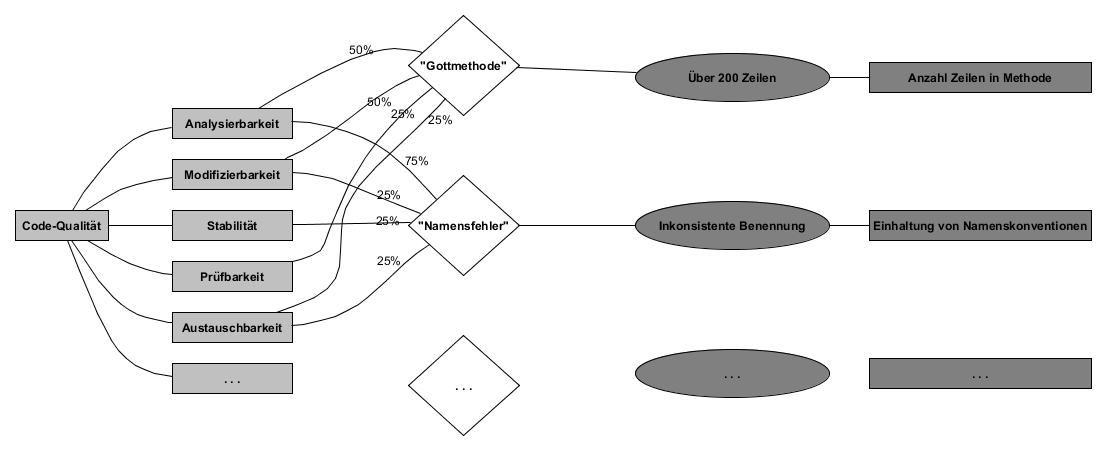
\includegraphics [width=\textwidth] {model.png}
				\caption{Ausschnitt des für den Code-Quality-Index verwendeten Qualitätsmodells mit Qualitätseigenschaften, Qualitätsindikatoren, Problemmustern und Qualitätsmerkmalen (von links nach rechts)}
				\label{qualitymodel}
			\end{figure}
			\subsection{Qualitätsindikatoren}
				Die 52 Qualitätsindikatoren aus denen sich der Index zusammensetzt enthalten also jeweils ein zugeordnetes Problemmuster als Definition, und die gewichtete Abbildung auf die Qualitätseigenschaften von null bis einhundert Prozent, wobei die Abstufung jeweils in 25 Prozent Schritten erfolgt. Darüber hinaus wurde für alle Indikatoren analysiert wie hoch der Aufwand zur Behebung des Problemmusters ist ("`Kostenzuwachs"') und wie unmittelbar sich eine Behebung positiv auswirkt. Beides wurde analog zur Skala für die Qualitätseigenschaften eingestuft. Abschließend wurden über 120 Industrieprojekte hinsichtlich der Problemmuster vermessen und die Ergebnisse in einer Datenbank abgelegt. Dabei wurden die Fehlerhäufigkeiten jeweils mittels der Anzahl der Codezeilen des vermessenen Systems normiert um vergleichbare Werte zu erhalten und so aufbereitet, dass sich ein neu zu untersuchendes System im Vergleich zu dieser Datenbasis einordnen lässt. Dafür wurde erneut auf die Abstufung in 25 Prozent Schritten zurückgegriffen, sodass sich bezüglich jedes Indikators aussagen lässt, ob das vermessene Programm besser als 25, 50, 75 oder 100 Prozent der Programme in der Datenbasis ist. Diese Grenzen werden als "`Schwellwerte"' bezeichnet. \newline
			Als Beispiel sei hier der Qualitätsindikator "`duplizierter Code"' aufgeführt, der folgendermaßen definiert ist \cite{CodeQualityManagement}:
				\begin{quote}
  					"`Duplizierter Code liegt vor, wenn mindestens 40 aufeinander folgende Codezeilen (inkl. Leerzeilen und Kommentarzeilen) innerhalb des Quellcodes in identischer Form mehrmals auftreten."'
  				\end{quote}
  				\begin{figure} [h]
					\centering
					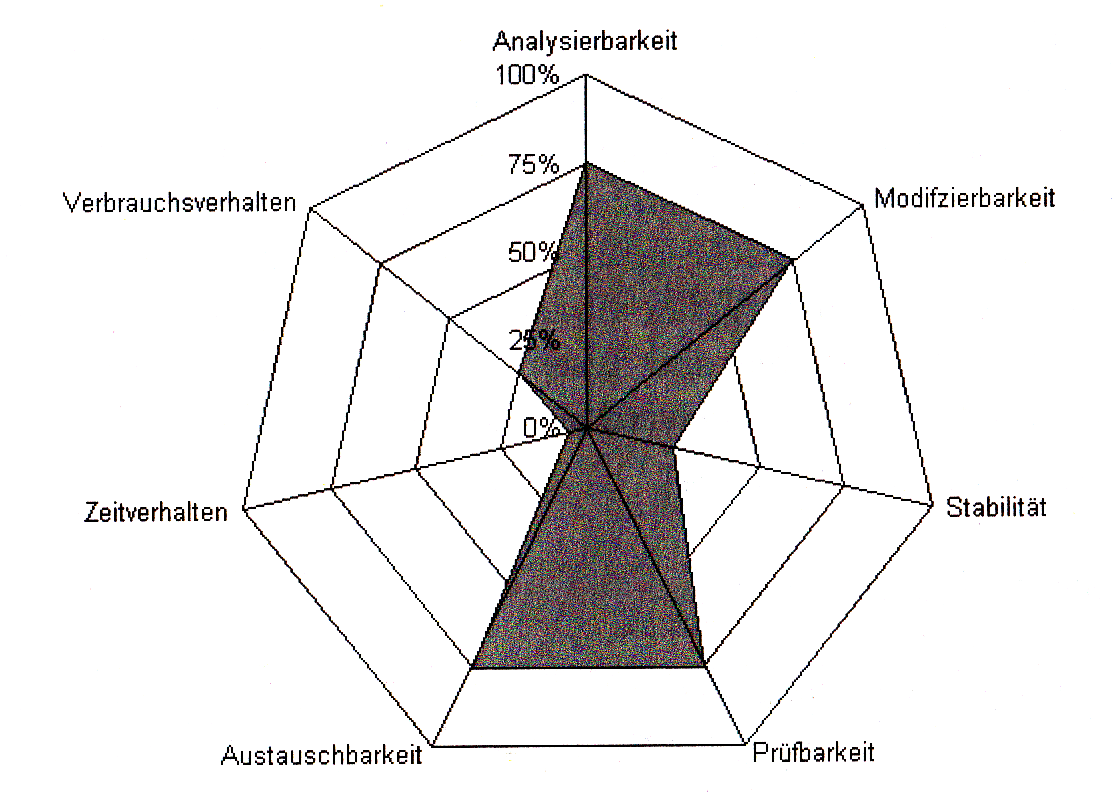
\includegraphics [width=0.6\textwidth] {indexeigenschaften.png}
					\caption{Zuordnung des Problemmusters "`duplizierter Code"' zu den Qualitätseigenschaften \cite{CodeQualityManagement}}
					\label{indexeigen}
				\end{figure}
				Die Zuordnung zu den Qualitätseigenschaften wird mittels Kiviatdiagramm dargestellt (siehe Abbildung~\ref{indexeigen}). Der Kostenzuwachs wurde mit 50 Prozent bewertet, die Unmittelbarkeit mit 75 Prozent. Abbildung~\ref{indexschwell} beinhaltet die Häufigkeit des Problemmusters in der Datenbasis (für Java-Programme). \newline
				\begin{figure} [h]
					\centering
					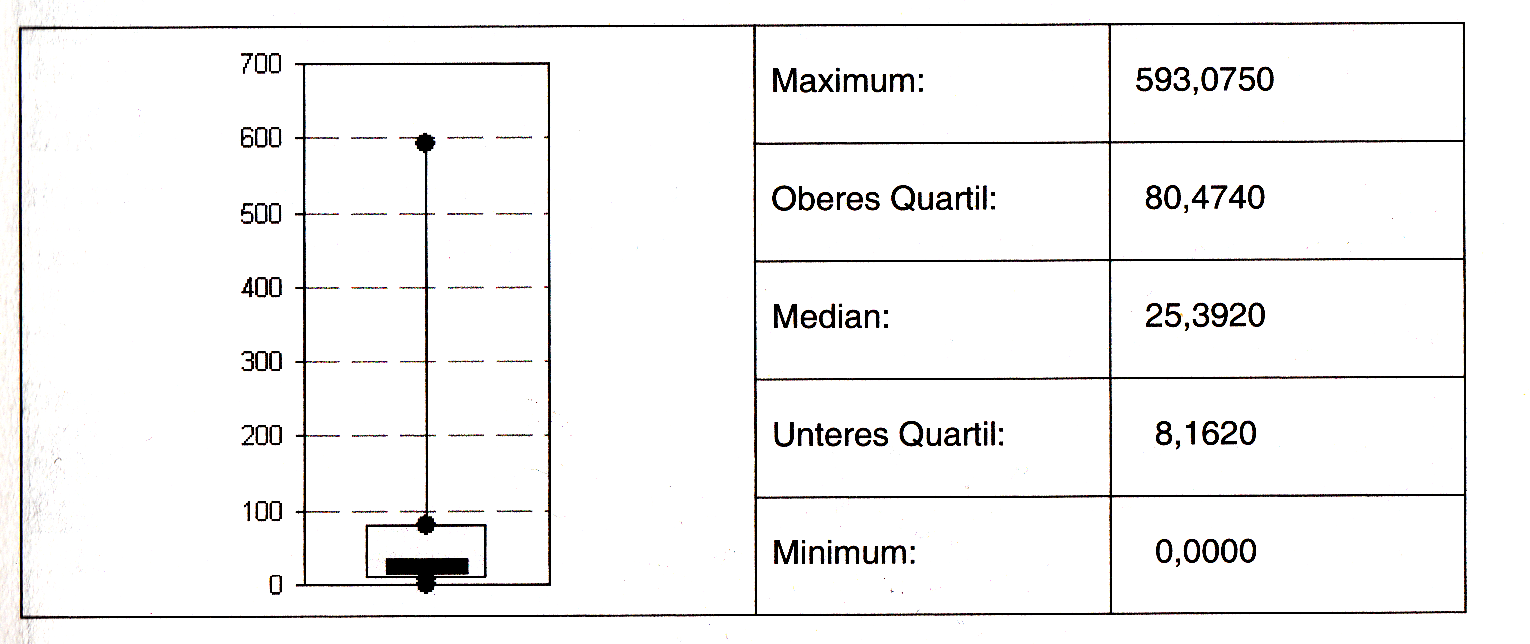
\includegraphics [width=\textwidth] {indexschwellwerte.png}
					\caption{Anzahl duplizierter Codezeilen je 1000 Zeilen Code in Datenbasis \cite{CodeQualityManagement}}
					\label{indexschwell}
				\end{figure}
			\subsection{Index-Definition}
				Um anhand der Messergebnisse für die Indikatoren eine Gesamteinstufung in Form eines einfachen Indexes zu ermöglichen wurden fünf Quality-Benchmark-Level (QBL) definiert (siehe Tabelle~\ref{indexlevel}) deren Erreichbarkeit über zwei Mechanismen gesteuert wird:
				\begin{itemize}
					\item \textbf{Indikatorzuwachs} Mit jedem Level kommen weitere Indikatoren hinzu, abhängig davon welche Qualitätseigenschaften sie beeinflussen. Je nach Kostenzuwachs und Unmittelbarkeit können Indikatoren darüber hinaus vorgezogen oder in höhere Level verschoben werden (unmittelbar wirkende, schnell zu korrigierende Indikatoren werden bevorzugt).
					\item \textbf{Schwellwerttunnel} Je höher der zu erreichende Level, desto besser muss das vermessene Programm im Vergleich zur Datenbasis für die relevanten Indikatoren abschneiden (25\% für QBL 2 bis 100\% für QBL 5). 
				\end{itemize}
				\begin{center}
					\tabulinesep=1.5mm
					\begin{longtabu}{|c|c|c|c|}
						\hline
  						\textbf{Level} & \textbf{Bezeichnung} & \textbf{Beschreibung} & \textbf{Eigenschaften} \\
  						\hline 
						QBL 1 & Rudimentary & komplierfähiges, ausführbares Programm & - \\  						
  						\hline
  						QBL 2 & Basic & Minimum an Code-Qualität für & Analysierbarkeit \\ & & wirtschaftliche Anpassbarkeit & Stabilität \\
  						\hline
  						QBL 3 & Extended & gute technische Qualität, & Zeitverhalten \\ & & technisch Zukunftsfähig & Verbrauchsverhalten \\
  						\hline
  						QBL 4 & Advanced & hervorragende Qualität, explizite & Prüfbarkeit \\ & & Struktur für Weiterentwicklung & Modifizierbarkeit \\
  						\hline
  						QBL 5 & Complete & perfekte Qualität, Struktur für & Austauschbarkeit \\ & & Weiterentwicklung und Wiederverwendung & \\
  						\hline
  						\caption{Für den Code-Quality-Index definierte Level \cite{CodeQualityManagement}}
						\label{indexlevel}
  					\end{longtabu}   
  				\end{center}
  				\newpage
		\section{Verwendung und Bewertung in der Praxis}
			Vorab lässt sich sagen, dass der Code-Quality-Index in dieser Form weder zu einem weitreichend akzeptiertem Standard geworden ist, noch vielfältige Anwendung in der Wirtschaft gefunden hat. Auch die von den Autoren angestrebte Fortführung der angefangenen Datenbasis ist anscheinend nicht langfristig durchgeführt worden. Der im Buch genannte Webauftritt ist nicht mehr erreichbar. \newline
			Allerdings gab es mindestens eine Umsetzung für ein produktives System. Für die IT-Infrastruktur der Dresdener Bank, also die Bereitstellung von Online-Funktionen und Informationen für Endkunden und Mitarbeiter innerhalb einer J2EE-Architektur wurde Code-Quality-Management in Form des beschriebenen Indexes durch die SQS AG etabliert und damit zufriedenstellende Ergebnisse erreicht \cite{DresdnerBank}. Allerdings wurde hierbei festgestellt, dass die Auswahl und konkrete Ausprägung der Indikatoren für den Kontext angepasst werden müssen. Die 52 Indikatoren von Frank Simon et Al. können nicht als allgemeingültig betrachtet werden. \newline
			Eine weniger praxisnahe aber vollständige Umsetzung des Code-Quality-Index erfolgte im Rahmen der Diplomarbeit von Torsten Möllenbeck an der Universität Bremen \cite{DAIndexUmsetzung}. Diese zeigt, dass es auf jeden Fall möglich ist, den Index vollständig automatisiert zu ermitteln, auch wenn leider nur Ergebnisse von C++ Programmen ausgewertet wurden. Allerdings werden einige Kritikpunkte an der Konzeption des Indexes angebracht, die ihre Berechtigung haben:
			\begin{itemize}
				\item Die dynamischen Schwellwerte abhängig von der Datenbasis können dazu führen, dass Systeme nachträglich anders eingestuft würden, wenn weitere besonders gute oder besonders schlechte Programme hinzugefügt werden. Mit Blick auf das Softwarepraktikum bedeutet dies, dass die Datenbasis zumindest über den Verlauf eines Softwarepraktikums konstant gehalten werden muss um eine gerechte und stabile Bewertung vorzunehmen und darüber hinaus die Entwicklung der Qualität im Verlauf des Praktikums zu untersuchen.
				\item Der Aufbau des Indexes kann dazu führen, dass ein System das bezüglich fast aller Indikatoren eine hervorragende Qualität aufweist aber in einem einzigen Indikator sehr schlecht ist, beziehungsweise bewusst von einer Regel abweicht auf dem untersten Level eingestuft wird. Es erscheint daher sinnvoll den Index Kontextspezifisch anzupassen wenn die Notwendigkeit besteht.
				\item Auch wenn die Problemmuster durch die Autoren gut belegt sind erscheinen einige der gewählten Grenzwerte recht willkürlich und damit auch fragwürdig. Als Beispiel sei hier der Indikator "`falsche Namenslänge"' genannt, bei dem es sicher verschiedene Meinungen zu der Frage gibt ob 50 Zeichen wirklich eine sinnvolle Grenze sind. Auch hier bietet sich eine spezifische Anpassung für das zu bewertende System an.
			\end{itemize}
			Trotz dieser Schwächen und dem nicht erfüllten Universalitätsanspruch finden sich einige Umsetzungen ähnlicher Bewertungssysteme. So wurde durch Ana Dragomir und Horst Lichter an der Universität Aachen ein Index für die Beurteilung von Softwarearchitekturen vorgeschlagen \cite{ArchitectureIndex}. \newline
			Ein sehr ähnliches vorgehen wie beim Code-Quality-Index verfolgen Baggen et Al. mit ihrem Code-Benchmark \cite{CodeBenchmark}. Es werden ebenso Indikatoren gebildet und auf beeinflusste Qualitätseigenschaften abgebildet, allerdings werden hier sehr viel weniger und allgemeinere Indikatoren verwendet. Ein etwas neuerer Ansatz aus der Wirtschaft stammt von der Firma TIOBE die mit ihrem TIOBE Quality Indicator ebenfalls weniger Indikatoren definieren als im Code-Quality-Index \cite{TIOBEIndex}. Allerdings werden für die erreichbaren Stufen keine Indikatoren ausgewählt sondern es werden immer alle vermessen. Unterschiedlich ist dabei dann lediglich der zu erreichende Schwellwert. Für die Gesamtbewertung wurde darüber hinaus noch eine Wichtung der Indikatoren vorgenommen. Als hervorstechendes Merkmal sei hier die ansprechende Präsentation des Ergebnisses genannt, dass an die Energieeffizienz-Plaketten von elektrischen Geräten erinnert (Siehe Abbildung~\ref{TIOBElabel}). \newline
			\begin{figure} [h]
				\centering
				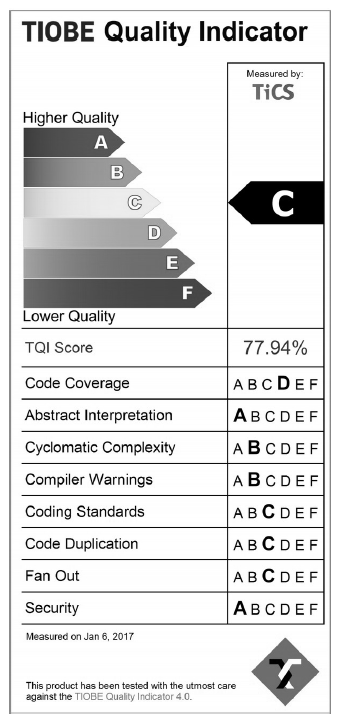
\includegraphics [width=0.4\textwidth] {tiobe.png}
				\caption{TIOBE Quality Indicator Ergebnisdarstellung \cite{TIOBEIndex}}
				\label{TIOBElabel}
			\end{figure}
		\section{Anpassung für das Softwarepraktikum}
			Die Anwendung des Code-Quality-Index in anderen Projekten und vergleichbare Ansätze machen ebenso deutlich wie die vom Indikatorkatalog abweichende Regelwerkdefinition, dass für das Softwarepraktikum der Code-Quality-Index nicht einfach übernommen werden kann, sondern entsprechend den speziellen Anforderungen und Möglichkeiten in diesem Rahmen angepasst werden muss. \newline
			Zunächst fällt auf, dass sich die gewählten Regeln nicht ohne weiteres auf das bidirektionale Qualitätsmodell von Simon et Al. abbilden lassen. Es müsste für die im Original nicht verwendeten Regeln aufwendig neu erforscht werden. Außerdem ist dieses Modell für die einführende Lehrveranstaltung zu komplex um es den Studenten erschöpfend zu vermitteln. Die Zuordnung der Regeln beziehungsweise Indikatoren als Mengen von Regeln zu einem Benchmark-Level muss daher über einen anderen Mechanismus erfolgen. Die einfachste und naheliegende Möglichkeit dafür bilden die Einstufungen der Regeln nach Schweregrad, sodass "`Blocker"'-Regeln bereits für den Level zwei und "`Info"'-Regeln erst für den Level vier relevant sind. Die Verschiebung der Regeln je nach Unmittelbarkeit und Kostenzuwachs entfällt in diesem Kontext vollständig, da dies ebenso neu ermittelt werden müsste und im Kontext des Softwarepraktikums mit dem gewählten Regelwerk ohnehin keine große Rolle spielt. \newline
			Eine weitere Anpassung betrifft die Schwellwerte. Da es in der Lehre nicht üblich ist für die beste Note 100 Prozent zu verlangen erscheint dies auch für den Code-Quality-Index als zu strenge Forderung. Daher wurde zusätzlich der Schwellwert "`Besser als 90\%"' eingeführt um eine adäquate Bewertung vorzunehmen. Tabelle~\ref{indexdef} enthält die mit dem Lehrstuhl abgestimmte Neudefinition der Benchmark-Level für das Softwarepraktikum. Da sich bei der Vermessung der Praktikumsprojekte der letzten 2 Jahrgänge herausstellte, dass diese Schwellwerte dazu führen, dass bis auf eine Gruppe alle nur Level eins erreichen und die Index-Einstufung so keine Aussagekraft haben kann wurden die Schwellwerte stattdessen in 10-Prozent-Schritten ermittelt und die Zuordnung zu den Benchmark-Level über die angelegte Datenbank konfigurierbar gemacht. Mit der in Tabelle~\ref{indexdefnew} festgelegten Zuordnung erreichen die Gruppen Einstufungen zwischen Level eins und Level vier. \newline 
			\begin{center}
				\tabulinesep=1.5mm
				\begin{longtabu}{|c|c|c|c|}
					\hline
  					\textbf{Level} & \textbf{Bezeichnung} & \textbf{Beschreibung} \\
  					\hline 
					QBL 1 & Mangelhaft & komplierfähiges, ausführbares Programm \\  						\hline
  					QBL 2 & Ausreichend & 50\% Blocker, 25\% Critical \\ 
  					\hline
  					QBL 3 & Befriedigend & 75\% Blocker, 50\% Critical, 50\% Major, 25\% Minor \\
  					\hline
  					QBL 4 & Gut & 90\% Blocker, 75\% Critical, 75\% Major, 50\% Minor, 50\% Info \\
  					\hline
  					QBL 5 & Sehr Gut & 100\% Blocker, 100\% Critical, 90\% Major, 90\% Minor, 90\% Info \\
  					\hline
  					\caption{Neudefinition der Benchmark-Level für das Softwarepraktikum vor der Vermessung}
					\label{indexdef}
  				\end{longtabu}   
  			\end{center}
  			\begin{center}
				\tabulinesep=1.5mm
				\begin{longtabu}{|c|c|c|c|}
					\hline
  					\textbf{Level} & \textbf{Bezeichnung} & \textbf{Beschreibung} \\
  					\hline 
					QBL 1 & Mangelhaft & komplierfähiges, ausführbares Programm \\  						\hline
  					QBL 2 & Ausreichend & 10\% Blocker \\ 
  					\hline
  					QBL 3 & Befriedigend & 20\% Blocker, 10\% Critical, 10\% Major \\
  					\hline
  					QBL 4 & Gut & 30\% Blocker, 30\% Critical, 20\% Major, 10\% Minor \\
  					\hline
  					QBL 5 & Sehr Gut & 50\% Blocker, 40\% Critical, 30\% Major, 20\% Minor, 10\% Info \\
  					\hline
  					\caption{Für die Vermessung verwendete Definition der Benchmark-Level, die eine Annehmbare Verteilung der Bewertungen erzeugt}
					\label{indexdefnew}
  				\end{longtabu}   
  			\end{center}
  			Dieses starke Herabsetzen der Grenzen zum Erreichen eines höheren Benchmark-Level ist notwendig, da in den vermessenen Projekten keine Gruppe dabei war, die bezüglich aller Indikatoren im oberen Bereich liegt. Die meisten Gruppen sind bezüglich einiger weniger Indikatoren sehr gut, dafür aber bezüglich der meisten anderen nur Mittelfeld. Interessanterweise sind die gut erfüllten Indikatoren nicht immer die Gleichen, sondern sehr unterschiedlich. Dadurch entstehen im Aufbau der Datenbank Anspruchsvolle Zielwerte für alle Indikatoren, die dann von keiner Gruppe bezüglich aller Indikatoren eingehalten werden. Wenn das neue Regelwerk in Zukunft kommuniziert und von den Studenten angewendet wird ist es möglich, dass eine nachträgliche Anpassung der Zuordnungen sinnvoll wird. \newline
  			Im Folgenden werden die definierten Indikatoren kurz vorgestellt. Die genannten SonarQube-Regeln finden sich in der Dokumentation des Java-Plugins \cite{JavaPlugin}. \newline
  			\subsection{Indikator Duplizierter Code}
  				Klasse: "`Blocker"' \newline
  				Entspricht der SonarQube-Regel "`Source files should not have any duplicated blocks"' wobei im Gegensatz zum Original-Index die Anzahl der duplizierten Code-Blöcke gezählt wird und nicht die Anzahl der darin enthaltenen Zeilen. 
  				\begin{center}
					\tabulinesep=1.5mm
					\begin{longtabu}{|c|c||c|c||c|c||c|c|}
						\hline
  						\textbf{Besser als} & \textbf{Häufigkeit je 1000 LOC} & 20\% & 2,230 & 50\% & 1,446 & 80\% & 0,717 \\
  						\hline 
						0\% & 3,454 & 30\% & 1,891 & 60\% & 1,181 & 90\% & 0,259 \\
  						\hline 
						10\% & 2,965 & 40\% & 1,605 & 70\% & 0,935 & 100\% & 0,000 \\
						\hline
  						\caption{Ermittelter Schwellwerttunnel für Indikator Duplizierter Code}
  					\end{longtabu}   
  				\end{center}
  			\subsection{Indikator Magic Numbers}
  				Klasse: "`Blocker"' \newline
  				Entspricht der SonarQube-Regel "`Magic numbers should not be used"' und hat im Original-Index keine Entsprechung. Aufgrund der im Softwarepraktikum verwendeten Daten-Initialisierung durch eine Klasse mit dem Prefix "`DataInitializer"' in der sehr viele Zahlen im Code stehen ohne das dies ein Problem darstellt werden die Regelverletzungen in diesen Klassen für den Index ignoriert.
  				\begin{center}
					\tabulinesep=1.5mm
					\begin{longtabu}{|c|c||c|c||c|c||c|c|}
						\hline
  						\textbf{Besser als} & \textbf{Häufigkeit je 1000 LOC} & 20\% & 16,248 & 50\% & 8,922 & 80\% & 2,677 \\
  						\hline 
						0\% & 79,771 & 30\% & 13,127 & 60\% & 6,890 & 90\% & 1,054 \\
  						\hline 
						10\% & 25,179 & 40\% & 11,275 & 70\% & 3,968 & 100\% & 0,000 \\
						\hline
  						\caption{Ermittelter Schwellwerttunnel für Indikator Magic Numbers}
  					\end{longtabu}   
  				\end{center}
  			\subsection{Indikator Datenkapselaufbruch}
  				Klasse: "`Blocker"' \newline
  				Entspricht der SonarQube-Regel "`Class variable fields should not have public accessibility"' und ist in seiner Bedeutung identisch zum Original.
  				\begin{center}
					\tabulinesep=1.5mm
					\begin{longtabu}{|c|c||c|c||c|c||c|c|}
						\hline
  						\textbf{Besser als} & \textbf{Häufigkeit je 1000 LOC} & 20\% & 0,836 & 50\% & 0,000 & 80\% & 0,000 \\
  						\hline 
						0\% & 6,430 & 30\% & 0,590 & 60\% & 0,000 & 90\% & 0,000 \\
  						\hline 
						10\% & 1,613 & 40\% & 0,178 & 70\% & 0,000 & 100\% & 0,000 \\
						\hline	
  						\caption{Ermittelter Schwellwerttunnel für Indikator Datenkapselaufbruch}
  					\end{longtabu}   
  				\end{center}
  			\subsection{Indikator Überbuchte Datei}
  				Klasse: "`Critical"' \newline
  				Entspricht der SonarQube-Regel "`Files should contain only one top-level class or interface each"' und ist in seiner Bedeutung identisch zum Original.
  				\begin{center}
					\tabulinesep=1.5mm
					\begin{longtabu}{|c|c||c|c||c|c||c|c|}
						\hline
  						\textbf{Besser als} & \textbf{Häufigkeit je 1000 LOC} & 20\% & 0,000 & 50\% & 0,000 & 80\% & 0,000 \\
  						\hline 
						0\% & 0,000 & 30\% & 0,000 & 60\% & 0,000 & 90\% & 0,000 \\
  						\hline 
						10\% & 0,000 & 40\% & 0,000 & 70\% & 0,000 & 100\% & 0,000 \\					
						\hline
  						\caption{Ermittelter Schwellwerttunnel für Indikator Überbuchte Datei}
  					\end{longtabu}   
  				\end{center}
  			\subsection{Indikator Unzureichende Tests}
  				Klasse: "`Critical"' \newline
  				Entspricht der SonarQube-Regel "`Lines should have sufficient coverage by unit tests"' und hat im Original-Index keine Entsprechung. Als ausreichende Testabdeckung wird im Kontext des Softwarepraktikums 80\% festgelegt. Dieser Grenzwert bewegt sich im Mittelfeld der in der Literatur genannten Werte und wurde vom Lehrstuhl so festgelegt. 
  				\begin{center}
					\tabulinesep=1.5mm
					\begin{longtabu}{|c|c||c|c||c|c||c|c|}
						\hline
  						\textbf{Besser als} & \textbf{Häufigkeit je 1000 LOC} & 20\% & 10,375 & 50\% & 7,976 & 80\% & 4,748 \\
  						\hline 
						0\% & 14,970 & 30\% & 9,708 & 60\% & 6,815 & 90\% & 2,893 \\
  						\hline 
						10\% & 13,109 & 40\% & 8,322 & 70\% & 6,217 & 100\% & 0,000 \\ 						
						\hline
  						\caption{Ermittelter Schwellwerttunnel für Indikator Unzureichende Tests}
  					\end{longtabu}   
  				\end{center}
  			\subsection{Indikator Zu enge Kopplung}
  				Klasse: "`Critical"' \newline
  				Enthält die beiden SonarQube-Regeln "`Classes should not be coupled to too many other classes (Single Responsibility Principle)"' und "`Cycles between packages should be removed"', wobei letztere dem Indikator "`Verbotene Paketliebe"' entspricht. Die enge thematische Zusammengehörigkeit führte zur Zusammenlegung. 
  				\begin{center}
					\tabulinesep=1.5mm
					\begin{longtabu}{|c|c||c|c||c|c||c|c|}
						\hline
  						\textbf{Besser als} & \textbf{Häufigkeit je 1000 LOC} & 20\% & 8,740 & 50\% & 6,554 & 80\% & 4,835 \\
  						\hline 
						0\% & 16,750 & 30\% & 7,133 & 60\% & 6,117 & 90\% & 3,978 \\
  						\hline 
						10\% & 10,256 & 40\% & 6,810 & 70\% & 5,606 & 100\% & 3,310 \\ 						
						\hline
  						\caption{Ermittelter Schwellwerttunnel für Indikator Zu enge Kopplung}
  					\end{longtabu}   
  				\end{center}
  			\subsection{Indikator Gottkonstrukt}
  				Klasse: "`Critical"' \newline
  				Enthält vier SonarQube-Regeln, die die Größe von Dateien, Klassen, Methoden und Inneren Klassen betreffen. Bis auf die Größe von inneren Klassen finden sich für alle Regeln entsprechende Qualitätsindikatoren. Da das übergeordnete Prinzip Code-Elemente klein und übersichtlich zu halten adressiert werden soll wurden diese zusammengelegt. Die Grenzwerte orientieren sich am Softwarepraktikum in Dortmund \cite{CleanCodeImPraktikum}.
  				\begin{center}
					\tabulinesep=1.5mm
					\begin{longtabu}{|c|c||c|c||c|c||c|c|}
						\hline
  						\textbf{Besser als} & \textbf{Häufigkeit je 1000 LOC} & 20\% & 8,326 & 50\% & 6,815 & 80\% & 5,615 \\
  						\hline 
						0\% & 9,422 & 30\% & 7,565 & 60\% & 6,591 & 90\% & 4,937 \\
  						\hline 
						10\% & 8,936 & 40\% & 7,253 & 70\% & 6,065 & 100\% & 3,960 \\						
						\hline
  						\caption{Ermittelter Schwellwerttunnel für Indikator Gottkonstrukt}
  					\end{longtabu}   
  				\end{center}
  				\newpage
  			\subsection{Indikator Informelle Dokumentation}
  				Klasse: "`Critical"' \newline
  				Entspricht der SonarQube-Regel "`Public types, methods and fields (API) should be documented with Javadoc"' und ist in seiner Bedeutung identisch zum Original.
  				\begin{center}
					\tabulinesep=1.5mm
					\begin{longtabu}{|c|c||c|c||c|c||c|c|}
						\hline
  						\textbf{Besser als} & \textbf{Häufigkeit je 1000 LOC} & 20\% & 44,137 & 50\% & 23,948 & 80\% & 8,854 \\
  						\hline 
						0\% & 63,249 & 30\% & 32,258 & 60\% & 21,304 & 90\% & 3,954 \\
  						\hline 
						10\% & 51,517 & 40\% & 25,868 & 70\% & 12,335 & 100\% & 0,000 \\  						
						\hline
  						\caption{Ermittelter Schwellwerttunnel für Indikator Informelle Dokumentation}
  					\end{longtabu}   
  				\end{center}
  			\subsection{Indikator Namensfehler} 
  				Klasse: "`Critical"' \newline
  				Enthält alle SonarQube-Regeln bezüglich Namenskonventionen und entspricht im wesentlichen dem Original. Die Standard-Java-Pattern wurden um die Größenbeschränkung gemäß dem Original-Indikator "`Falsche Namenslänge"' erweitert. Eine separate Messung dieses Indikators ist mit den vordefinierten Java-Regeln in SonarQube nicht möglich. 
  				\begin{center}
					\tabulinesep=1.5mm
					\begin{longtabu}{|c|c||c|c||c|c||c|c|}
						\hline
  						\textbf{Besser als} & \textbf{Häufigkeit je 1000 LOC} & 20\% & 27,724 & 50\% & 13,559 & 80\% & 6,969 \\
  						\hline 
						0\% & 57,931 & 30\% & 21,749 & 60\% & 11,245 & 90\% & 5,347 \\
  						\hline 
						10\% & 38,099 & 40\% & 14,811 & 70\% & 9,592 & 100\% & 1,123 \\					
						\hline
  						\caption{Ermittelter Schwellwerttunnel für Indikator Namensfehler}
  					\end{longtabu}   
  				\end{center}
  			\subsection{Indikator Zu Komplex}
  				Klasse: "`Major"' \newline
  				Enthält SonarQube-Regeln zur Verschachtelungstiefe von Kontrollflussanweisungen, Parameteranzahl von Methoden sowie die McCabe-Komplexität für Methoden und Klassen. Die Original-Indikatoren "`Labyrinthmethode"' und "`Lange Parameterliste"' sind Teil dieses Indikators.
  				\begin{center}
					\tabulinesep=1.5mm
					\begin{longtabu}{|c|c||c|c||c|c||c|c|}
						\hline
  						\textbf{Besser als} & \textbf{Häufigkeit je 1000 LOC} & 20\% & 9,251 & 50\% & 6,890 & 80\% & 3,881 \\
  						\hline 
						0\% & 20,474 & 30\% & 8,276 & 60\% & 6,054 & 90\% & 3,208 \\
  						\hline 
						10\% & 11,787 & 40\% & 7,376 & 70\% & 5,039 & 100\% & 2,109 \\						
						\hline
  						\caption{Ermittelter Schwellwerttunnel für Indikator Zu Komplex}
  					\end{longtabu}   
  				\end{center}
  			\subsection{Indikator Verwechslungsgefahr}
  				Klasse: "`Major"' \newline
  				Enthält alle SonarQube-Regeln, die die Überdeckung von Bezeichnern in untergeordneten Geltungsbereichen verbieten, sowie die Forderung, dass sich Bezeichner nicht nur in Groß- und Kleinschreibung unterscheiden dürfen und dass ein Datentyp-Suffix wie "`L"' für Long groß geschrieben werden soll. All diese Regeln haben zum Ziel Verwechslungen zu vermeiden. 
  				\begin{center}
					\tabulinesep=1.5mm
					\begin{longtabu}{|c|c||c|c||c|c||c|c|}
						\hline
  						\textbf{Besser als} & \textbf{Häufigkeit je 1000 LOC} & 20\% & 1,497 & 50\% & 0,356 & 80\% & 0,000 \\
  						\hline 
						0\% & 17,839 & 30\% & 0,554 & 60\% & 0,278 & 90\% & 0,000 \\
  						\hline 
						10\% & 2,687 & 40\% & 0,494 & 70\% & 0,000 & 100\% & 0,000 \\					
						\hline
  						\caption{Ermittelter Schwellwerttunnel für Indikator Verwechslungsgefahr}
  					\end{longtabu}   
  				\end{center}
  			\subsection{Indikator Formatierungsfehler}
  				Klasse: "`Major"' \newline
  				Enthält SonarQube-Regeln bezüglich der Setzung von geschweiften Klammern, Einrückung und Zeilenlänge. Keine der ausgewählten Regeln hat eine Entsprechung im Original Index.
  				\begin{center}
					\tabulinesep=1.5mm
					\begin{longtabu}{|c|c||c|c||c|c||c|c|}
						\hline
  						\textbf{Besser als} & \textbf{Häufigkeit je 1000 LOC} & 20\% & 232,493 & 50\% & 200,345 & 80\% & 149,972 \\
  						\hline 
						0\% & 288,193 & 30\% & 222,187 & 60\% & 183,627 & 90\% & 51,639 \\
  						\hline 
						10\% & 243,131 & 40\% & 209,668 & 70\% & 173,311 & 100\% & 0,000 \\						
						\hline
  						\caption{Ermittelter Schwellwerttunnel für Indikator Formatierungsfehler}
  					\end{longtabu}   
  				\end{center}
  			\subsection{Indikator Objektplacebo}
  				Klasse: "`Minor"' \newline
  				Entspricht der SonarQube-Regel "`"static" members should be accessed statically"' und ist in seiner Bedeutung identisch zum Original.\begin{center}
					\tabulinesep=1.5mm
					\begin{longtabu}{|c|c||c|c||c|c||c|c|}
						\hline
  						\textbf{Besser als} & \textbf{Häufigkeit je 1000 LOC} & 20\% & 0,000 & 50\% & 0,000 & 80\% & 0,000 \\
  						\hline 
						0\% & 6,366 & 30\% & 0,000 & 60\% & 0,000 & 90\% & 0,000 \\
  						\hline 
						10\% & 0,277 & 40\% & 0,000 & 70\% & 0,000 & 100\% & 0,000 \\						
						\hline
  						\caption{Ermittelter Schwellwerttunnel für Indikator Objektplacebo}
  					\end{longtabu}   
  				\end{center}
  			\subsection{Indikator Objektvergleich}
  				Klasse: "`Minor"' \newline
  				Entspricht der SonarQube-Regel "`Objects should be compared with equals()"' und hat im Original-Index keine Entsprechung.
  				\begin{center}
					\tabulinesep=1.5mm
					\begin{longtabu}{|c|c||c|c||c|c||c|c|}
						\hline
  						\textbf{Besser als} & \textbf{Häufigkeit je 1000 LOC} & 20\% & 1,248 & 50\% & 0,216 & 80\% & 0,000 \\
  						\hline 
						0\% & 4,970 & 30\% & 0,777 & 60\% & 0,000 & 90\% & 0,000 \\
  						\hline 
						10\% & 2,673 & 40\% & 0,503 & 70\% & 0,000 & 100\% & 0,000 \\						
						\hline
  						\caption{Ermittelter Schwellwerttunnel für Indikator Objektvergleich}
  					\end{longtabu}   
  				\end{center}
  			\subsection{Indikator Risikocode}
  				Klasse: "`Minor"' \newline
  				Enthält die beiden SonarQube-Regeln "`switch statements should end with default clauses"' und "`Switch cases should end with an unconditional break statement"'. Damit werden zwei drittel des Original-Indikators abgedeckt.
  				\begin{center}
					\tabulinesep=1.5mm
					\begin{longtabu}{|c|c||c|c||c|c||c|c|}
						\hline
  						\textbf{Besser als} & \textbf{Häufigkeit je 1000 LOC} & 20\% & 0,433 & 50\% & 0,000 & 80\% & 0,000 \\
  						\hline 
						0\% & 6,609 & 30\% & 0,182 & 60\% & 0,000 & 90\% & 0,000 \\
  						\hline 
						10\% & 0,948 & 40\% & 0,000 & 70\% & 0,000 & 100\% & 0,000 \\				
						\hline
  						\caption{Ermittelter Schwellwerttunnel für Indikator Risikocode}
  					\end{longtabu}   
  				\end{center}
  			\subsection{Indikator Importfehler}
  				Klasse: "`Minor"' \newline
  				Enthält die beiden SonarQube-Regeln "`Useless imports should be removed"' und "`Wildcard imports should not be used"'. Damit stellt dieser Indikator eine Mischung, aber nicht vollständige Abdeckung der Original-Indikatoren "`Importlüge"' und "`Importchaos"' dar.
  				\begin{center}
					\tabulinesep=1.5mm
					\begin{longtabu}{|c|c||c|c||c|c||c|c|}
						\hline
  						\textbf{Besser als} & \textbf{Häufigkeit je 1000 LOC} & 20\% & 13,312 & 50\% & 3,559 & 80\% & 0,000 \\
  						\hline 
						0\% & 40,994 & 30\% & 9,169 & 60\% & 1,593 & 90\% & 0,000 \\
  						\hline 
						10\% & 20,185 & 40\% & 4,853 & 70\% & 0,665 & 100\% & 0,000 \\
						\hline
  						\caption{Ermittelter Schwellwerttunnel für Indikator Importfehler}
  					\end{longtabu}   
  				\end{center}
			\subsection{Indikator Deklarationsfehler}
				Klasse: "`Minor"' \newline
				Enthält die Forderungen nach expliziter Deklaration der Sichtbarkeit, Deklaration so spät wie möglich und nur einer Variablendeklaration pro Anweisung. Es gibt keine Entsprechung im Original-Index.
				\begin{center}
					\tabulinesep=1.5mm
					\begin{longtabu}{|c|c||c|c||c|c||c|c|}
						\hline
  						\textbf{Besser als} & \textbf{Häufigkeit je 1000 LOC} & 20\% & 4,812 & 50\% & 2,494 & 80\% & 1,038 \\
  						\hline 
						0\% & 15,164 & 30\% & 3,924 & 60\% & 1,783 & 90\% & 0,000 \\
  						\hline 
						10\% & 8,603 & 40\% & 3,029 & 70\% & 1,386 & 100\% & 0,000 \\	
						\hline
  						\caption{Ermittelter Schwellwerttunnel für Indikator Deklarationsfehler}
  					\end{longtabu}   
  				\end{center}
			\subsection{Indikator Toter Code}
				Klasse: "`Minor"' \newline
				Enthält alle SonarQube-Regeln die das entfernen von ungenutzten Code-Elementen fordern und schließt damit die Original-Indikatoren "`Tote Attribute"', "`Tote Implementierung"' und "`Tote Methoden"' mit ein.
				\begin{center}
					\tabulinesep=1.5mm
					\begin{longtabu}{|c|c||c|c||c|c||c|c|}
						\hline
  						\textbf{Besser als} & \textbf{Häufigkeit je 1000 LOC} & 20\% & 7,560 & 50\% & 3,427 & 80\% & 1,262 \\
  						\hline 
						0\% & 36,247 & 30\% & 5,810 & 60\% & 2,941 & 90\% & 0,499 \\
  						\hline 
						10\% & 8,897 & 40\% & 3,978 & 70\% & 2,495 & 100\% & 0,178 \\	
						\hline
  						\caption{Ermittelter Schwellwerttunnel für Indikator Toter Code}
  					\end{longtabu}   
  				\end{center}
			\subsection{Indikator Unfertiger Code}
				Klasse: "`Info"' \newline
				Enthält neben der Forderung des Original-Indikators "`TODO"'-Tags zu entfernen zusätzlich die SonarQube-Regel "`Sections of code should not be commented out"'.
				\begin{center}
					\tabulinesep=1.5mm
					\begin{longtabu}{|c|c||c|c||c|c||c|c|}
						\hline
  						\textbf{Besser als} & \textbf{Häufigkeit je 1000 LOC} & 20\% & 10,456 & 50\% & 4,701 & 80\% & 1,386 \\
  						\hline 
						0\% & 62,675 & 30\% & 6,581 & 60\% & 2,900 & 90\% & 0,527 \\
  						\hline 
						10\% & 18,413 & 40\% & 5,992 & 70\% & 1,841 & 100\% & 0,000 \\	
						\hline
  						\caption{Ermittelter Schwellwerttunnel für Indikator Unfertiger Code}
  					\end{longtabu}   
  				\end{center}
		\section{Umsetzung in SonarQube}
			Die ursprüngliche Idee, den Index mittels der in der SonarQube-Web-Oberfläche definierbaren Quality-Gates abzubilden lies sich leider nicht umsetzen. Die Quality-Gates bieten zwar die Möglichkeit die Projekte hinsichtlich eines Maximalwertes für die Verletzung von Regeln der verschiedenen Stufen separat zu überprüfen \cite{QualityGates}, allerdings ist die Umsetzung des Indexes damit trotzdem nicht sinnvoll:
			\begin{itemize}
				\item Die Grenzwerte müssten fest angegeben werden und können nicht dynamisch aus einer Datenbasis generiert oder übernommen werden. Damit müsste die ermittelte Datenbasis manuell übertragen, und für die folgenden Jahre auch manuell angepasst werden.
				\item Ein Projekt lässt sich nur hinsichtlich eines Quality-Gates vermessen. Es müsste also pro Benchmark-Level jedes Projekt mit dem dazu passenden Quality-Gate vermessen werden um die erreichte Stufe manuell daraus abzuleiten.
			\end{itemize}
			Beide Umstände führen zu einer deutlichen Reduktion der angestrebten Automatisierung, sodass von dieser Idee abgerückt wurde und eine Umsetzung innerhalb des zu erweiternden Plugins erfolgte. Dafür wurde eine weitere Implementierung der SonarQube-Schnittstelle "`Decorator"' genutzt, in der Zugriff auf die ermittelten Fehlerzahlen besteht. \newline
			Da die Ermittlung des Indexes im Vergleich zu den zuvor vermessenen Projekten, also der Datenbasis erfolgt wurde zusätzlich zur von SonarQube genutzten Datenbank ein weiteres Datenbankschema angelegt, in dem die gemessenen Regelverletzungen nach Indikator gruppiert und mittels Netto-Code-Zeilen normiert abgelegt werden. Da es um eine konstante Bewertung der Gruppen im Verlaufe des Softwarepraktikums zu gewährleisten sinnvoll erscheint die Datenbasis konstant zu halten kann das Plugin bezüglich des Code-Quality-Index in zwei Modi betrieben werden. 
			\begin{itemize}
				\item Im Verlaufe des Praktikums wird lediglich die Einstufung der vermessenen Programme gegen die konstante Datenbasis vorgenommen. Es werden keine Messwerte in der Datenbank abgelegt, sodass die Schwellwerte sich mit besser oder schlechter werdenden Programmen nicht verschieben.
				\item Nach Abschluss eines Praktikumsjahrgangs sollten alle fertiggestellten Programme im zweiten Modus erneut vermessen werden, in dem statt der Einstufung des Programms eine Ablage der gemessenen Regelverletzungen in der Datenbasis und eine Neuberechnung der Schwellwerte erfolgt. Diese ergänzte Datenbasis soll dann der Vergleichswert für den kommenden Jahrgang sein und muss gegebenenfalls durch eine Anpassung der Benchmark-Level-Grenzen ergänzt werden, um eine sinnvolle Einstufung der Programme zu erhalten.	
			\end{itemize}		
  	\backmatter
  
  	\appendix
  	\bibliography{diplombib}
  
\end{document}
